\chapter{Results}
\label{Chap4}
\section{Powder ageing}

\subsection{Grain size and distribution}
\label{RGSAD}

The evolution of powder size distribution during the year, measured without any prior ultrasonic treatment, is available in figure \ref{fig:granulo}. Each plotted curve was averaged based on four measurements. The mean diameter ($D_a$) varied between 31.5 and 36.8 [$\mu$m], corresponding respectively to the last and first samplings. The standard deviation (SD) stayed between 14.8 and 16.2 [$\mu$m]. Details for the samplings conditions are available  in table \ref{tab:detcyc}. The grain size testing method demonstrated high reproducibility. For each sample, the curves for the four measurements seemed to overlap perfectly when observed at the scale of figure \ref{fig:granulo}.\\%Maximal absolute gaps of only 0.18 [$\mu$m] and 0.34 [$\mu$m] were measured for the values of $D_a$ and SD for two distributions of a same sample.\\

\begin{figure}[ht]
	\centering
	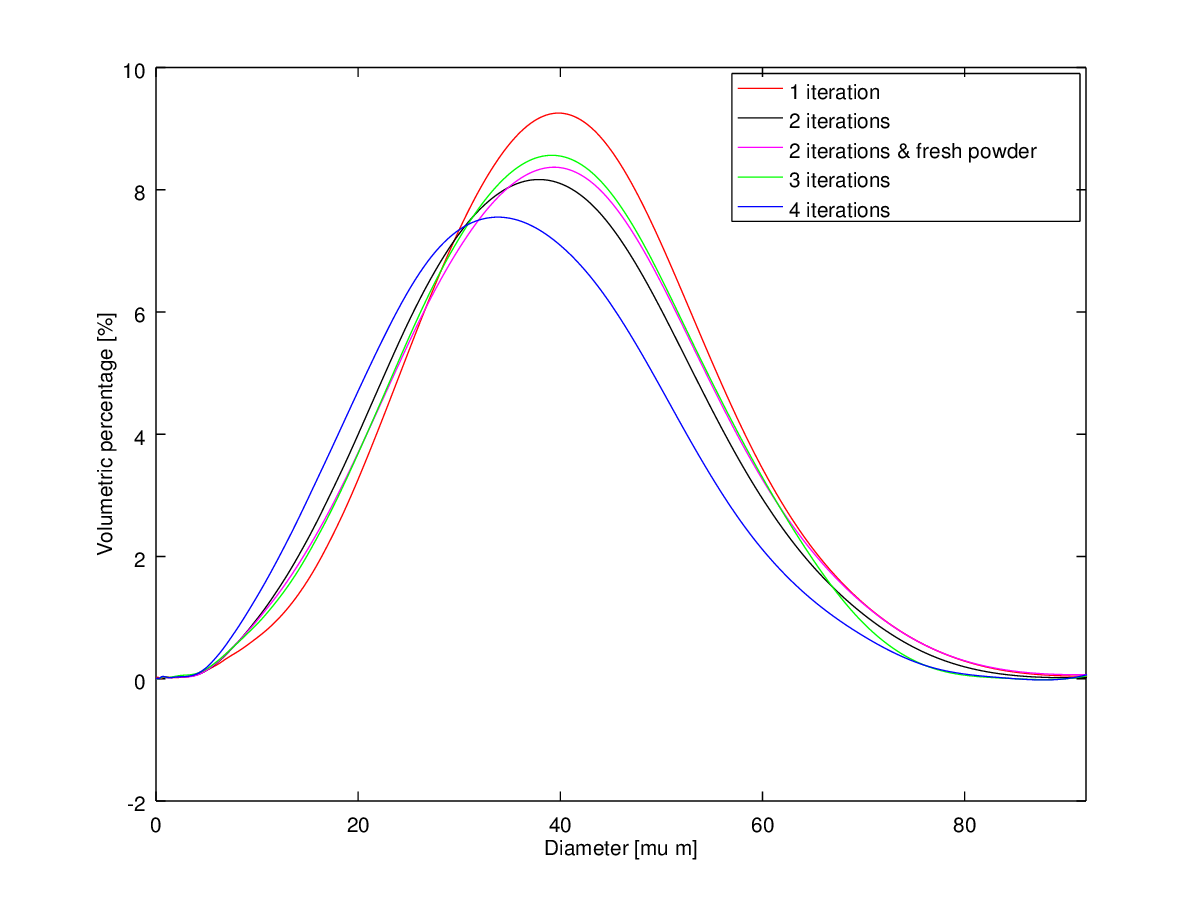
\includegraphics[scale=0.73]{Images/Granulo}
	\decoRule
	\caption[Evolution of powder size distributions with recycling iterations before ultrasonic treatments.]{Evolution of powder size distributions with recycling iterations before ultrasonic treatments.}
	\label{fig:granulo}
\end{figure}

%volumetric percentage

 \begin{center}
\begin{table}[ht]
\noindent\makebox[\textwidth]{\begin{tabular}{|c|c |c |c|}
    \hline
    Date of sampling& Number of recycling iterations& Prior addition of fresh powder & Batches\\
\hline 
\hline   
    23/10/2017 & 1 & No & X200-171024\\
    09/01/2018 & 2 & No & X200-180109\\
    21/02/2018 & 2 & Yes &X200-180220\\
    13/03/2018 & 3 & No& X200-180313\\
    &&&X200-180315\\
    &&&X200-180319\\
    17/04/2018 & 4 & No& X200-180417\\
    \hline
\end{tabular}}

\caption[Powder samplings recycling history]{Powder samplings recycling history}
\label{tab:detcyc}
\end{table}
 \end{center}

Mean diameters and standard deviations were compared before and after exposure to ultrasounds (US). Results are gathered in table \ref{tab:BAUS} with the 95\% confidence intervals (CI). In both cases, a general progressive decrease of the mean diameter and a narrowing of the distribution was observed as functions of the number of recycling cycles. The only exception to this trend is the distribution for February sample. This particular sampling was made the day after fresh powder was added to the recycled one. US caused a systematic decrease of $\simeq 10\%$ for $D_a$, exception made for the April sampling (only $6\%$). Ultrasonic treatment permitted to lower the maximal diameter measured from 134 to 84 [$\mu m$].  \\

 \begin{center}
\begin{table}[ht]
\noindent\makebox[\textwidth]{\begin{tabular}{|c|c |c |c| c|}
    \hline
    Date of sampling& \multicolumn{2}{c}{Before US} \vline & \multicolumn{2}{c}{After US} \vline\\
    \cline{2-5}
    & $D_a$& SD & $D_a$& SD\\
\hline 
\hline   
    23/10/2017  &36.8$\pm 0.1$ & 15.5$\pm 0.0$& 33.3 $\pm 0.0$ & 14.6$\pm 0.0$\\
    09/01/2018 &34.5$\pm 0.1$ &15.5 $\pm 0.1$&31.4 $\pm 0.0$  &14.6 $\pm 0.0$\\
    21/02/2018 &35.5$\pm 0.2$ & 16.2 $\pm 0.3$ & 32.1$\pm 0.1$ &14.9$\pm 0.0$\\
    13/03/2018 &35.0$\pm 0.0$ &15.2$\pm 0.0$ &31.6 $\pm 0.1$ & 14.5 $\pm 0.0$\\
    17/04/2018&31.5$\pm 0.1$ &14.8$\pm 0.0$ &29.6$\pm 0.0$&14.3 $\pm 0.0$\\
    \hline
\end{tabular}}

\caption[Average powder diameter and standard deviation before and after ultrasonic treatment]{Average powder diameter and standard deviation before and after ultrasonic treatment}
\label{tab:BAUS}
\end{table}
 \end{center}

\subsection{Composition}

\subsubsection{Fresh powder}

The composition of fresh (unrecycled) powder measured by ICP spectrometry is shown in table \ref{tab:compoF}. Each mass fraction is vitiated by a relative error than can go up to 3\%. The method thus gives far more precise results for elements in smaller quantities.\\
 \begin{center}
\begin{table}[ht]
\centering
\begin{tabular}{|c|c |c |c| }
    \hline
    %\multicolumn{4}{c}{Composition [\%wt]} \vline \\
    Al [\%wt]& Fe [\%wt]&Mg [\%wt]&Si [\%wt]\\
\hline 
\hline   
    89.0 $\pm 2.67$&0.14 $\pm 0.004$& 0.50 $\pm 0.015$ &9.99 $\pm 0.300$\\
    \hline
\end{tabular}

\caption[Composition of the fresh AlSi10Mg powder]{Composition of the fresh AlSi10Mg powder}
\label{tab:compoF}
\end{table}
 \end{center}


\subsubsection{Recycled powder}

The reiterations of this analysis on the recycled powder used for different batches gave the results in table \ref{tab:compo}. The samples tested were the same as for the grain sizes analysis (see table \ref{tab:detcyc}). Mass fractions as a function of time are displayed on figure \ref{fig:Compo}, with the corresponding error bars. There appears to be a peak of alloying elements mass fractions for February sample. It seems that these quantities drop progressively the following two months. However, these assertions should be taken with a grain of salt due to the large error bars.

\begin{figure}[ht]
\centering
\noindent\makebox[\textwidth]{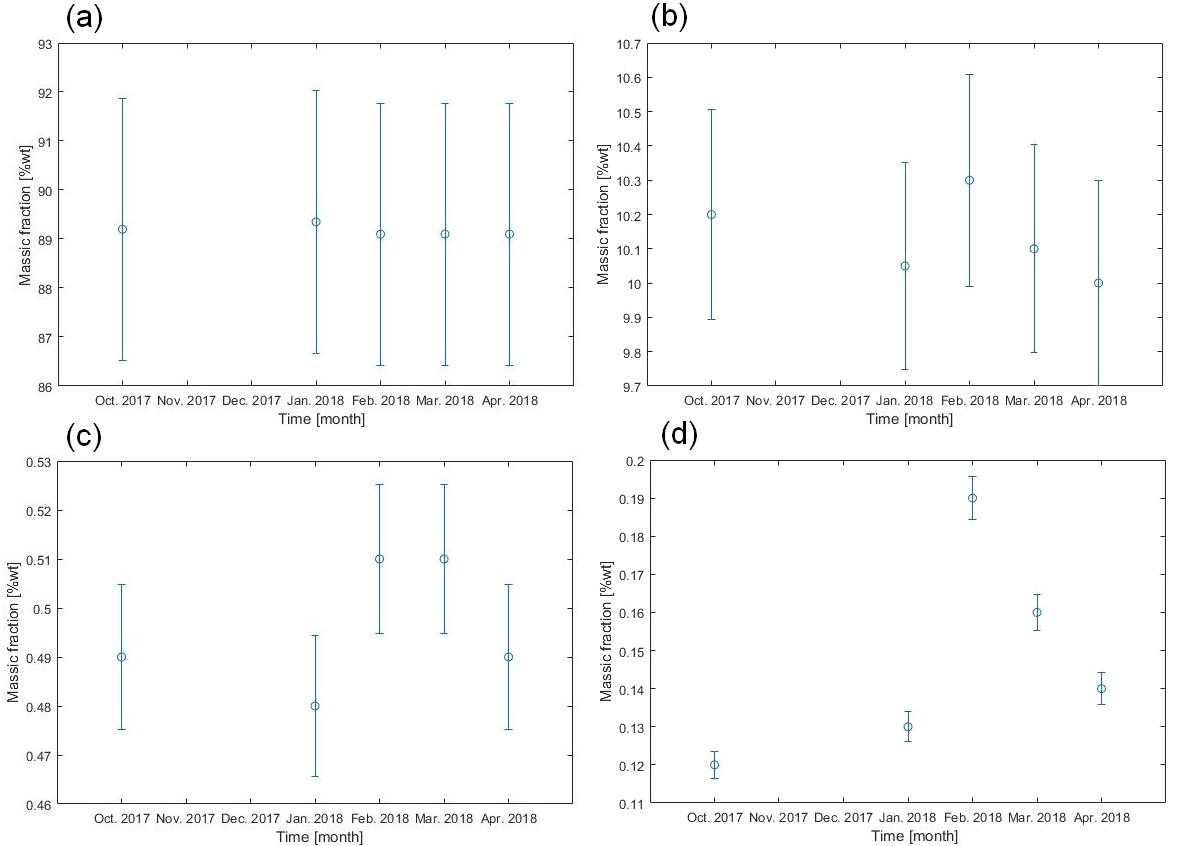
\includegraphics[scale=0.5]{Images/Compo}}
\decoRule
\caption[Evolution of concentration of the recycled powder constituting elements: (a) aluminium mass fraction (b) silicon mass fraction (c) magnesium mass fraction (d) iron mass fraction]{Evolution of concentration of the recycled powder constituting elements: (a) aluminium mass fraction (b) silicon mass fraction (c) magnesium mass fraction (d) iron mass fraction}
\label{fig:Compo}
\end{figure} 


 \begin{center}
\begin{table}[ht]
\noindent\makebox[\textwidth]{\begin{tabular}{|c|c |c |c| c|}
    \hline
    Date of sampling& \multicolumn{4}{c}{Composition [\%wt]} \vline\\
    \cline{2-5}
    & Al& Fe&Mg&Si\\
\hline 
\hline   
    23/10/2017  &89.2 $\pm 2.67$&0.12 $\pm 0.004$&0.49 $\pm 0.015$&10.2$\pm 0.3$\\
    09/01/2018 & 89.3  $\pm 2.67$& 0.13$\pm 0.004$ &0.48$\pm 0.014$&10.1$\pm 0.3$\\
    %12/01/2018 & 89.4  $\pm 2.68$& 0.13$\pm 0.004$ &0.48$\pm 0.014$&10.0$\pm 0.3$\\
    21/02/2018&89.1 $\pm 2.67$&0.19$\pm 0.006$&0.51$\pm 0.015$&10.3$\pm 0.3$\\
    13/03/2018 &89.1  $\pm 2.67$&0.16$\pm 0.005$&0.51$\pm 0.015$&10.1$\pm 0.3$\\    
    17/04/2018& 89.1  $\pm 2.67$&0.14$\pm 0.004$& 0.49 $\pm 0.015$ &10.0$\pm 0.3$\\
    \hline
\end{tabular}}

\caption[Composition of recycled AlSi10Mg powder as a function of the date]{Composition of recycled AlSi10Mg powder as a function of the date}
\label{tab:compo}
\end{table}
 \end{center}

\subsubsection{SLM processed material}

Two samples of batch X200-171024 were machined in order to extract material chips to use for ICP analysis. The composition after completion of the SLM process could thus  be compared with the original one (sampled the 23/10/2017). Table \ref{tab:chip} shows the results for both. A relative loss of a few percent was measured for magnesium (between 3.5\% and 4.7 \%). It seems that the mass fraction of silicon also decreased (of $\simeq 1\%$) but this is uncertain due to the large error bars. \\

 \begin{center}
\begin{table}[ht]
\centering
\begin{tabular}{|c|c|c |c |c| }
    \hline
    Sample& \multicolumn{4}{c}{Composition [\%wt]} \vline\\
    \cline{2-5}
    & Al& Fe&Mg&Si\\
\hline 
\hline   
    5 & 89.6 $\pm 2.67$&0.13 $\pm 0.004$& 0.47 $\pm 0.015$ &9.89 $\pm 0.300$\\
        7 & 89.5$\pm 2.67$&0.12 $\pm 0.004$& 0.48 $\pm 0.015$ &9.90 $\pm 0.300$\\
    \hline
\end{tabular}

\caption[Compositions of the chips extracted from samples "5" and "7" from batch X200-171024]{Compositions of the chips extracted from samples "5" and "7" from batch X200-171024}
\label{tab:chip}
\end{table}
 \end{center}



\section{Density and hardness study}
\subsection{Optimisation of the SLM parameters}
\label{Rparaopti}
The optimisation of the manufactured samples properties was done with respect to $\rho_{a,rel}$ and $H_v$. For this purpose, twelve cubes were fabricated with P varying from 75\% $P_{max} $ to $P_{max}$ and $v_s$ from 900 to 1500 [$\frac{mm}{sec}$]. Details about batch X200-171024 are given in appendix \ref{AppendixA}. The goal of this optimisation was to select a single set of parameters values to use in the rest of the thesis. The parameters values were chosen to cover a wide range of $E_d$. Sets of parameters ($P=75\% P_{max}$ ; $v_s=1200 [\frac{mm}{sec}]$) and ($P=75\% P_{max}$ ; $v_s=900 [\frac{mm}{sec}]$) gave the best results in terms of $\rho_{a,rel}$ in a previous study done at UCL. It was decided to produce samples with these sets of values in triplicate in order to have a first insight on the process reproducibility. This will be discussed further in next section. Here, only the mean $H_v$ and $\rho_{a,rel}$ of those samples will be compared to the others.\\

Results for the measurements of $\rho_{a,rel}$ and $H_v$ are summarised in figure \ref{fig:HD2-171024} and detailed in appendix \ref{AppendixA}. The 95\% confidence intervals (CI) are drawn on the graphs. The methods used to compute them are described in appendix \ref{AppendixC}. All apparent relative density values were obtained through hydrostatic weighing of the unpolished AB specimens.\\

\begin{figure}[ht]
\centering
\noindent\makebox[\textwidth]{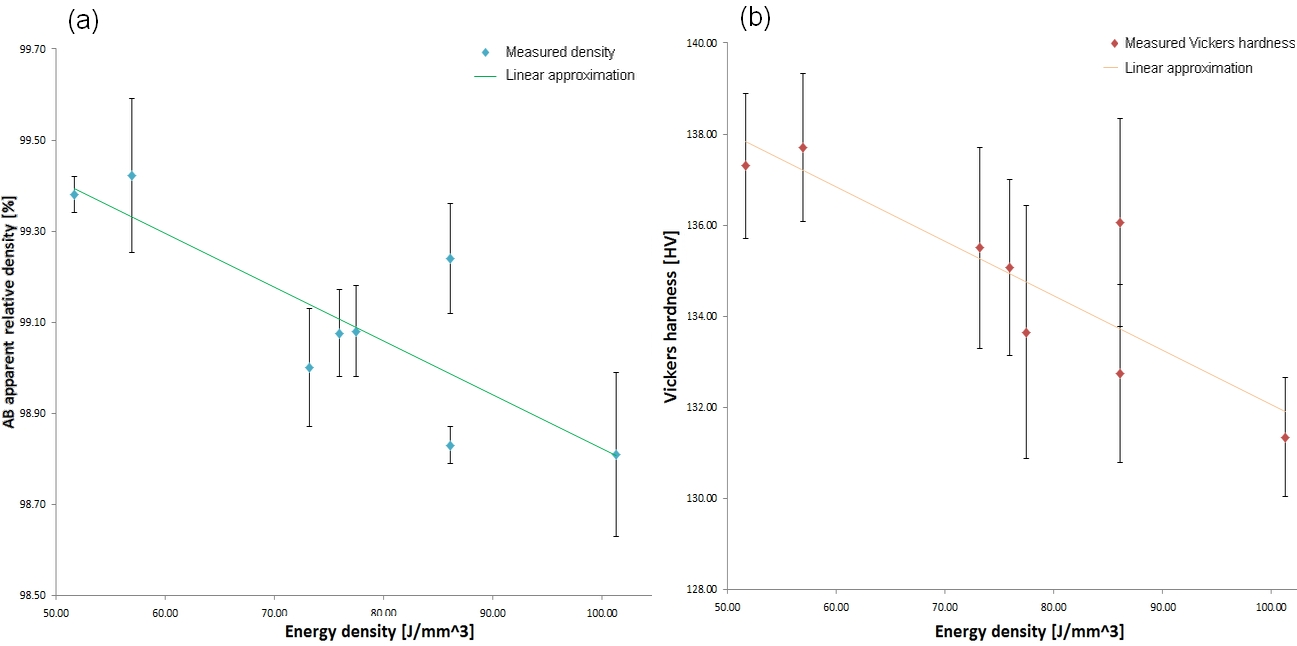
\includegraphics[scale=0.5]{Images/HD2-171024}}
\decoRule
\caption[Batch X200-171024 samples properties as a function of the energy density: (a) as-built apparent relative density (b) Vickers hardness]{Batch X200-171024 samples properties as a function of the energy density: (a) as-built apparent relative density (b) Vickers hardness}
\label{fig:HD2-171024}
\end{figure} 

Both $\rho_{a,rel}$ and $H_v$ reached maximal values for ($P=75\% P_{max}$ ; $v_s=1200 [\frac{mm}{sec}]$). It was thus chosen to work with this optimal set of parameters values in the rest of the thesis. The graph then shows a general progressive decrease of  $\rho_{a,rel}$ and $H_v$ for $E_d>57 [\frac{J}{mm^3}]$. Two samples were fabricated using the same energy density ($E_d \simeq 86.1$) but with different P and $v_s$. The lower density and hardness at this $E_d$ value on graph \ref{fig:HD2-171024} both correspond to the parameters values ($P=P_{max}$ ; $v_s=1059 [\frac{mm}{sec}]$).


\subsection{Reproducibility}
\label{RReprod}
%\subsubsection{Relative density and hardness}
\subsubsection{General results}
Batch X200-171024 raised a reproducibility issue. Sample "8a", fabricated with parameters ($P=75\% P_{max}$ ; $v_s=900 [\frac{mm}{sec}]$), had a relative density $\simeq 5 [\%]$ lower than the others' ($\rho_{a,rel}=98.77[\%]$). It was decided to produce a batch of fifteen ($P=75\% P_{max}$ ; $v_s=1200 [\frac{mm}{sec}]$) cubic samples and fifteen ($P=75\% P_{max}$ ; $v_s=900 [\frac{mm}{sec}]$) others in order to assess the process reproducibility when using a same powder. It was chosen to work with the two sets of parameters to compare the results for optimal and sub-optimal set values, and to try understanding the conditions that caused the poor properties sample "8a". Part of the samples were fabricated closely to one another (see \ref{fig:180109-real}) to see if the specimens rapprochement has any effect on their final properties. The distance between two adjacent cubes in the same row (that is quasi-aligned with y) was $\simeq 50 [mm]$. The distance separating the rows was $\simeq 70 [mm]$. The apparent relative density was once more measured with the unpolished AB samples.\\

 \begin{center}
\begin{table}[ht]
\noindent\makebox[\textwidth]{\begin{tabular}{|c|c|c |c |c|}
    \hline
    Type & $\overline{\rho_{a,rel}}$ [\%] & $SD_{\rho_{a,rel}}$[\%]& $\overline{H_v}$ [HV]& $SD_{H_v}$[HV]\\

\hline
\hline   
    ($P=75\% P_{max}$ ; $v_s=1200 [\frac{mm}{sec}]$) & 99.42 & 0.08 & 138 & 0.4 \\
    ($P=75\% P_{max}$ ; $v_s=900 [\frac{mm}{sec}]$) & 99.08 & 0.27 & 135 & 1.3 \\
\hline

\end{tabular}}

\caption[Average values and standard deviations for apparent relative densities and hardnesses of the specimens of batch X200-171024]{Average values and standard deviations for apparent relative densities and hardnesses of the specimens of batch X200-171024}
\label{tab:78}
\end{table}
 \end{center}

Hardness and apparent relative density results for batch X200-180109 are shown in appendix \ref{AppendixA}. The key information is displayed in tables \ref{tab:78b} and \ref{tab:78bb}. Type ($P=75\% P_{max}$ ; $v_s=900 [\frac{mm}{sec}]$) samples exhibited slightly poorer properties than type ($P=75\% P_{max}$ ; $v_s=1200 [\frac{mm}{sec}]$) ones in average. However, the former have far better properties to what one could have expected based on previous results (see table \ref{tab:78}). The highest measured density is 99.54 [\%].\\

%\begin{figure}[ht]
%\centering
%\centerline{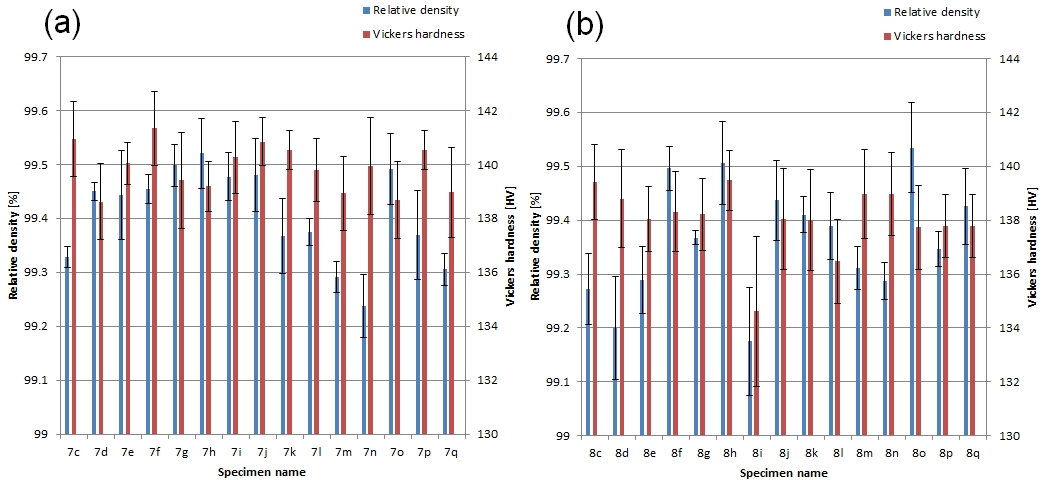
\includegraphics[scale=0.65]{Images/HD-180109-both}}
%\decoRule
%\caption[As-built apparent relative density and hardness results of batch X200-180109 for (a) type ($P=75\% P_{max}$ ; $v_s=1200 [\frac{mm}{sec}]$) samples (b) type ($P=75\% P_{max}$ ; $v_s=900 [\frac{mm}{sec}]$) samples.]{As-built apparent relative density and hardness results of batch X200-180109 for (a) type ($P=75\% P_{max}$ ; $v_s=1200 [\frac{mm}{sec}]$) samples (b) type ($P=75\% P_{max}$ ; $v_s=1200 [\frac{mm}{sec}]$) samples.}
%\label{fig:HD-171024}
%\end{figure} 



 \begin{center}
\begin{table}[ht]
\noindent\makebox[\textwidth]{\begin{tabular}{|c|c|c |c |c|}
    \hline
    Type & $\overline{\rho_{a,rel}}$ [\%] & $SD_{\rho_{a,rel}}$[\%]& $\overline{H_v}$ [HV]& $SD_{H_v}$[HV]\\

\hline
\hline   
    ($P=75\% P_{max}$ ; $v_s=1200 [\frac{mm}{sec}]$) & 99.40 & 0.09 & 139.9 & 0.87 \\
    ($P=75\% P_{max}$ ; $v_s=900 [\frac{mm}{sec}]$) & 99.36 & 0.11 & 138.3 & 1.3 \\


\hline
\end{tabular}}

\caption[Average values and standard deviations for apparent relative densities and hardnesses of the specimens of batch X200-180109]{Average values and standard deviations for apparent relative densities and hardnesses of types the specimens of batch X200-180109}
\label{tab:78b}
\end{table}
 \end{center}
 
 
 \begin{center}
\begin{table}[ht]
\noindent\makebox[\textwidth]{\begin{tabular}{|c|c|c |c |c|}
    \hline
    Type & $min(\rho_{a,rel})$ [\%] & $max(\rho_{a,rel})$[\%]& $ min(H_v)$ [HV]& $max(H_v)$[HV]\\

\hline
\hline   
    ($P=75\% P_{max}$ ; $v_s=1200 [\frac{mm}{sec}]$)  & 99.24 & 99.52 & 138.6 & 141.4 \\
    ($P=75\% P_{max}$ ; $v_s=900 [\frac{mm}{sec}]$) & 99.18 & 99.54 & 134.6 & 140.4 \\


\hline
\end{tabular}}

\caption[Minimal and maximal values for apparent relative densities and hardnesses of the specimens of batch X200-180109]{Minimal and maximal values for apparent relative densities and hardnesses of the specimens of batch X200-180109}
\label{tab:78bb}
\end{table}
 \end{center}

\subsubsection{Sample proximity and position influence}
The results are displayed in figure \ref{fig:180109-HD} as functions of the (x,y) positions of the samples on the manufacturing plate. The coordinates are such that the roll sweeps were done in the positive $x$ direction during the fabrication. Other graphs showing the averaged $\rho_{a,rel}$ and $H_v$ as functions of the x and y coordinates were also plotted. The samples distanced from less than 1 [cm] along x or y were considered to have the same corresponding coordinate. The graphs are shown in appendix \ref{AppendixD}. No significant trend was observed on these graphs: the variations of hardnesses and relative densities are too small compared to the CI. \\
\begin{figure}[h!]
\centering
\centerline{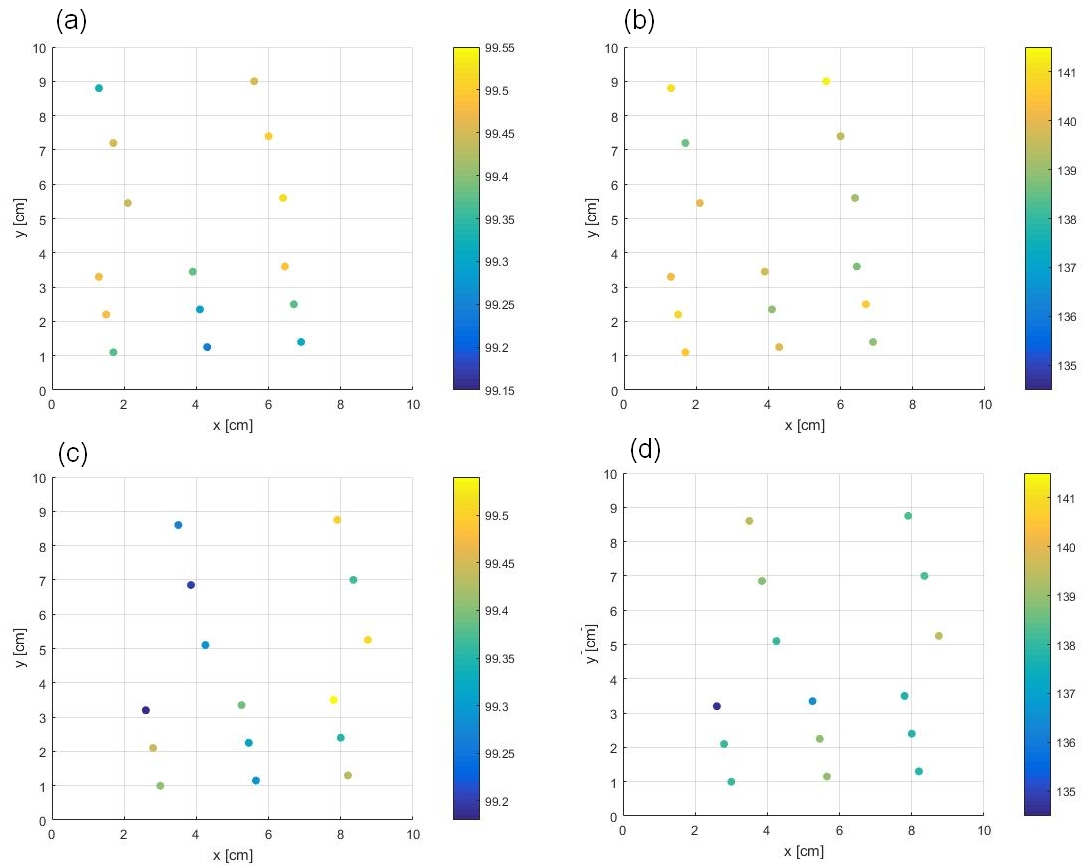
\includegraphics[scale=0.62]{Images/180109-HD}}
\decoRule
\caption[Batch X200-180109 scatter plots as functions of the (x,y) position on the manufacturing plate: (a) type (P=0.75 $Pmax$; $v_s$=1200 $\frac{mm}{sec}$) apparent relative densities (b) type (P=0.75 $Pmax$; $v_s$=1200 $\frac{mm}{sec}$) hardnesses (c) type (P=0.75 $Pmax$; $v_s$=900 $\frac{mm}{sec}$) apparent relative densities (d) type (P=0.75 $Pmax$; $v_s$=900 $\frac{mm}{sec}$) hardnesses]{Batch X200-180109 scatter plots as functions of the (x,y) position on the manufacturing plate: (a) type (P=0.75 $Pmax$; $v_s$=1200 $\frac{mm}{sec}$) apparent relative densities (b) type (P=0.75 $Pmax$; $v_s$=1200 $\frac{mm}{sec}$) hardnesses (c) type (P=0.75 $Pmax$; $v_s$=900 $\frac{mm}{sec}$) apparent relative densities (d) type (P=0.75 $Pmax$; $v_s$=900 $\frac{mm}{sec}$) hardnesses}
\label{fig:180109-HD}
\end{figure} 

A comparison of the results for closely packed samples (y<6) and distant ones (y>6) was also carried out. The details are shown in tables \ref{tab:CPD} and  \ref{tab:CPD2}. Again, no significant distinction could be drawn between the two.

 \begin{center}
\begin{table}[ht]
\noindent\makebox[\textwidth]{\begin{tabular}{|c|c|c|c |c |c|}
    \hline
    Type & Position& $\overline{\rho_{a,rel}}$ [\%] & $SD_{\rho_{a,rel}}$[\%]& $\overline{H_v}$ [HV]& $SD_{H_v}$[HV]\\

\hline
\hline   
    ($P=75\% P_{max}$ ; $v_s=1200 [\frac{mm}{sec}]$) & y>6& 99.45 & 0.07 & 140.0 & 1.1 \\
         & y<6& 99.38 & 0.07 & 139.9 & 0.7 \\
    ($P=75\% P_{max}$ ; $v_s=900 [\frac{mm}{sec}]$) & y>6& 99.36 & 0.10 & 138.7 & 0.6 \\
    & y<6& 99.37 & 0.08 & 138.0 & 1.6 \\


\hline
\end{tabular}}

\caption[Average values and standard deviations for apparent relative densities and hardnesses of the specimens of batch X200-180109, with distinction between the closely packed samples and the others]{Average values and standard deviations for apparent relative densities and hardnesses of types the specimens of batch X200-180109, with distinction between the closely packed samples and the others}
\label{tab:CPD}
\end{table}
 \end{center}
 
 
 \begin{center}
\begin{table}[ht]
\noindent\makebox[\textwidth]{\begin{tabular}{|c|c|c |c |c|c|}
    \hline
    Type & Position & $min(\rho_{a,rel})$ [\%] & $max(\rho_{a,rel})$[\%]& $ min(H_v)$ [HV]& $max(H_v)$[HV]\\

\hline
\hline   
    ($P=75\% P_{max}$ ; $v_s=1200 [\frac{mm}{sec}]$)&y>6 & 99.33 & 99.52 & 138.6 & 141.4 \\
    &y<6 & 99.24 & 99.49 & 138.7 & 140.9 \\
    ($P=75\% P_{max}$ ; $v_s=900 [\frac{mm}{sec}]$) &y>6& 99.20 & 99.51 & 138.0 & 139.5 \\
    &y<6& 99.29 & 99.54 & 134.6 & 140.4 \\


\hline
\end{tabular}}

\caption[Minimal and maximal values for apparent relative densities and hardnesses of the specimens of batch X200-180109]{Minimal and maximal values for apparent relative densities and hardnesses of the specimens of batch X200-180109}
\label{tab:CPD2}
\end{table}
 \end{center}

\subsubsection{Scan order influence}
The apparent relative densities, Vickers hardnesses and the corresponding 95 \% CI are displayed as functions of the scan order in figure \ref{fig:180109-SO}. The period of time between two successive scans of powder layers is the same for every sample. However, the time span between the scan and the powder covering differs from one to the other. This could lead to differences in terms of thermal exchanges.\\

\begin{figure}[ht]
\centering
\centerline{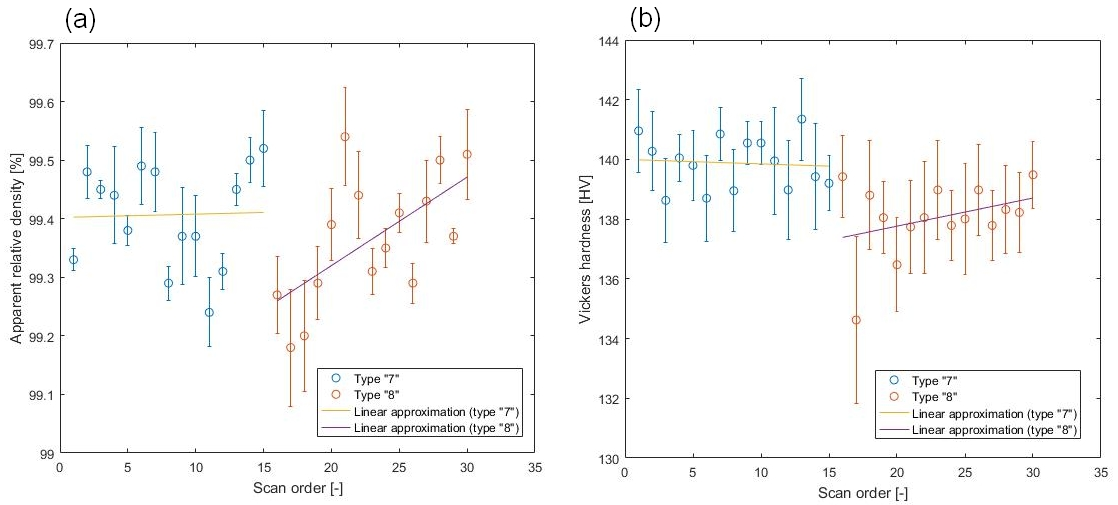
\includegraphics[scale=0.62]{Images/180109-SO}}
\decoRule
\caption[Batch X200-180109 scatter plots as functions of the scan order of (a) the apparent relative densities (b) the Vickers hardnesses]{Batch X200-180109 scatter plots as functions of the scan order of (a) the apparent relative densities (b) the Vickers hardnesses}
\label{fig:180109-SO}
\end{figure} 

Only one trend can be noted: the density of the ($P=75\% P_{max}$ ; $v_s=900 [\frac{mm}{sec}]$) samples appears to be larger for later scanning. However, this doesn't help understanding the poorer properties measured for samples with the same parameters in batch X200-171024 as they were precisely the last scanned. \\

\subsubsection{Powder influence}
\label{RPI}
The hardnesses and relative densities of samples manufactured using the optimised parameters ($P=75\% P_{max}$ ; $v_s=1200 [\frac{mm}{sec}]$) were monitored throughout this whole work. In this way, it was possible to study the impact of the powder ageing. Control cubes of dimensions 10x10x10 [$mm^3$] were produced in multiple batches for that purpose. The average measurements for those samples are gathered in table \ref{tab:control}. Detailed information is given in appendix \ref{AppendixA}.\\

 \begin{center}
\begin{savenotes}
 \begin{table}[ht]
\noindent\makebox[\textwidth]{\begin{tabular}{|c|c|c |c |c|}
    \hline
    Batch & $\overline{\rho_{a,rel}}$ \footnote{Measured by HW (AB)} [\%]  & $\overline{\rho_{a,rel}}$ \footnote{Measured by HW (polished)} [\%]  & $\overline{\rho_{rel}}$ \footnote{Measured by RODIA} [\%]  & $\overline{H_v}$ [HV]\\

\hline
\hline   
    X200-171024&99.42 & - & - & 137.7 \\
    X200-180109&99.40 & 99.51  & 99.59 & 139.9 \\
    X200-180319&- &  99.75  & 99.84 & 139.8 \\
    X200-180417&- &  99.47  & 99.67 & 136.0 \\
\hline
\end{tabular}}

\caption[Average hardness and relative density measurements for the control cubes of each batch]{Average hardness and relative density measurements for the control cubes of each batch}
\label{tab:control}
\end{table}
\end{savenotes}
 \end{center}

Samples from batches X200-180222 and X200-180228 are not included in this section. In those cases, fresh steamed powder was used, which induced high porosity in the produced parts. The most reasonable explanation is that the powder processing caused the formation of aggregates. This was not investigated further, and only recycled powder was employed thereafter. Table \ref{tab:control} indicates that the relative density peaked with batch X200-170319. It dropped slightly afterwards with batch X200-170417. Hardness also decreased - more significantly - with this last batch.\\

\subsubsection{Melt pools sizes and distribution study}
\label{rs_mps}

Samples "8a" and "8b" of batch X200-171024 were fabricated using the same manufacturing parameters. However, the former had way lower $\rho_{a,rel}$ and $H_v$ (see appendix \ref{AppendixA}). A statistical analysis of the melt pools size distribution was conducted for both samples to try grasping a better understanding of the origin of the differences. The procedure described in section \ref{MMOM} was followed. 130 zones were manually delineated for both samples. An illustration of the zones subdivision is shown on figure \ref{fig:B1}.\\

\begin{figure}[ht]
\centering
\centerline{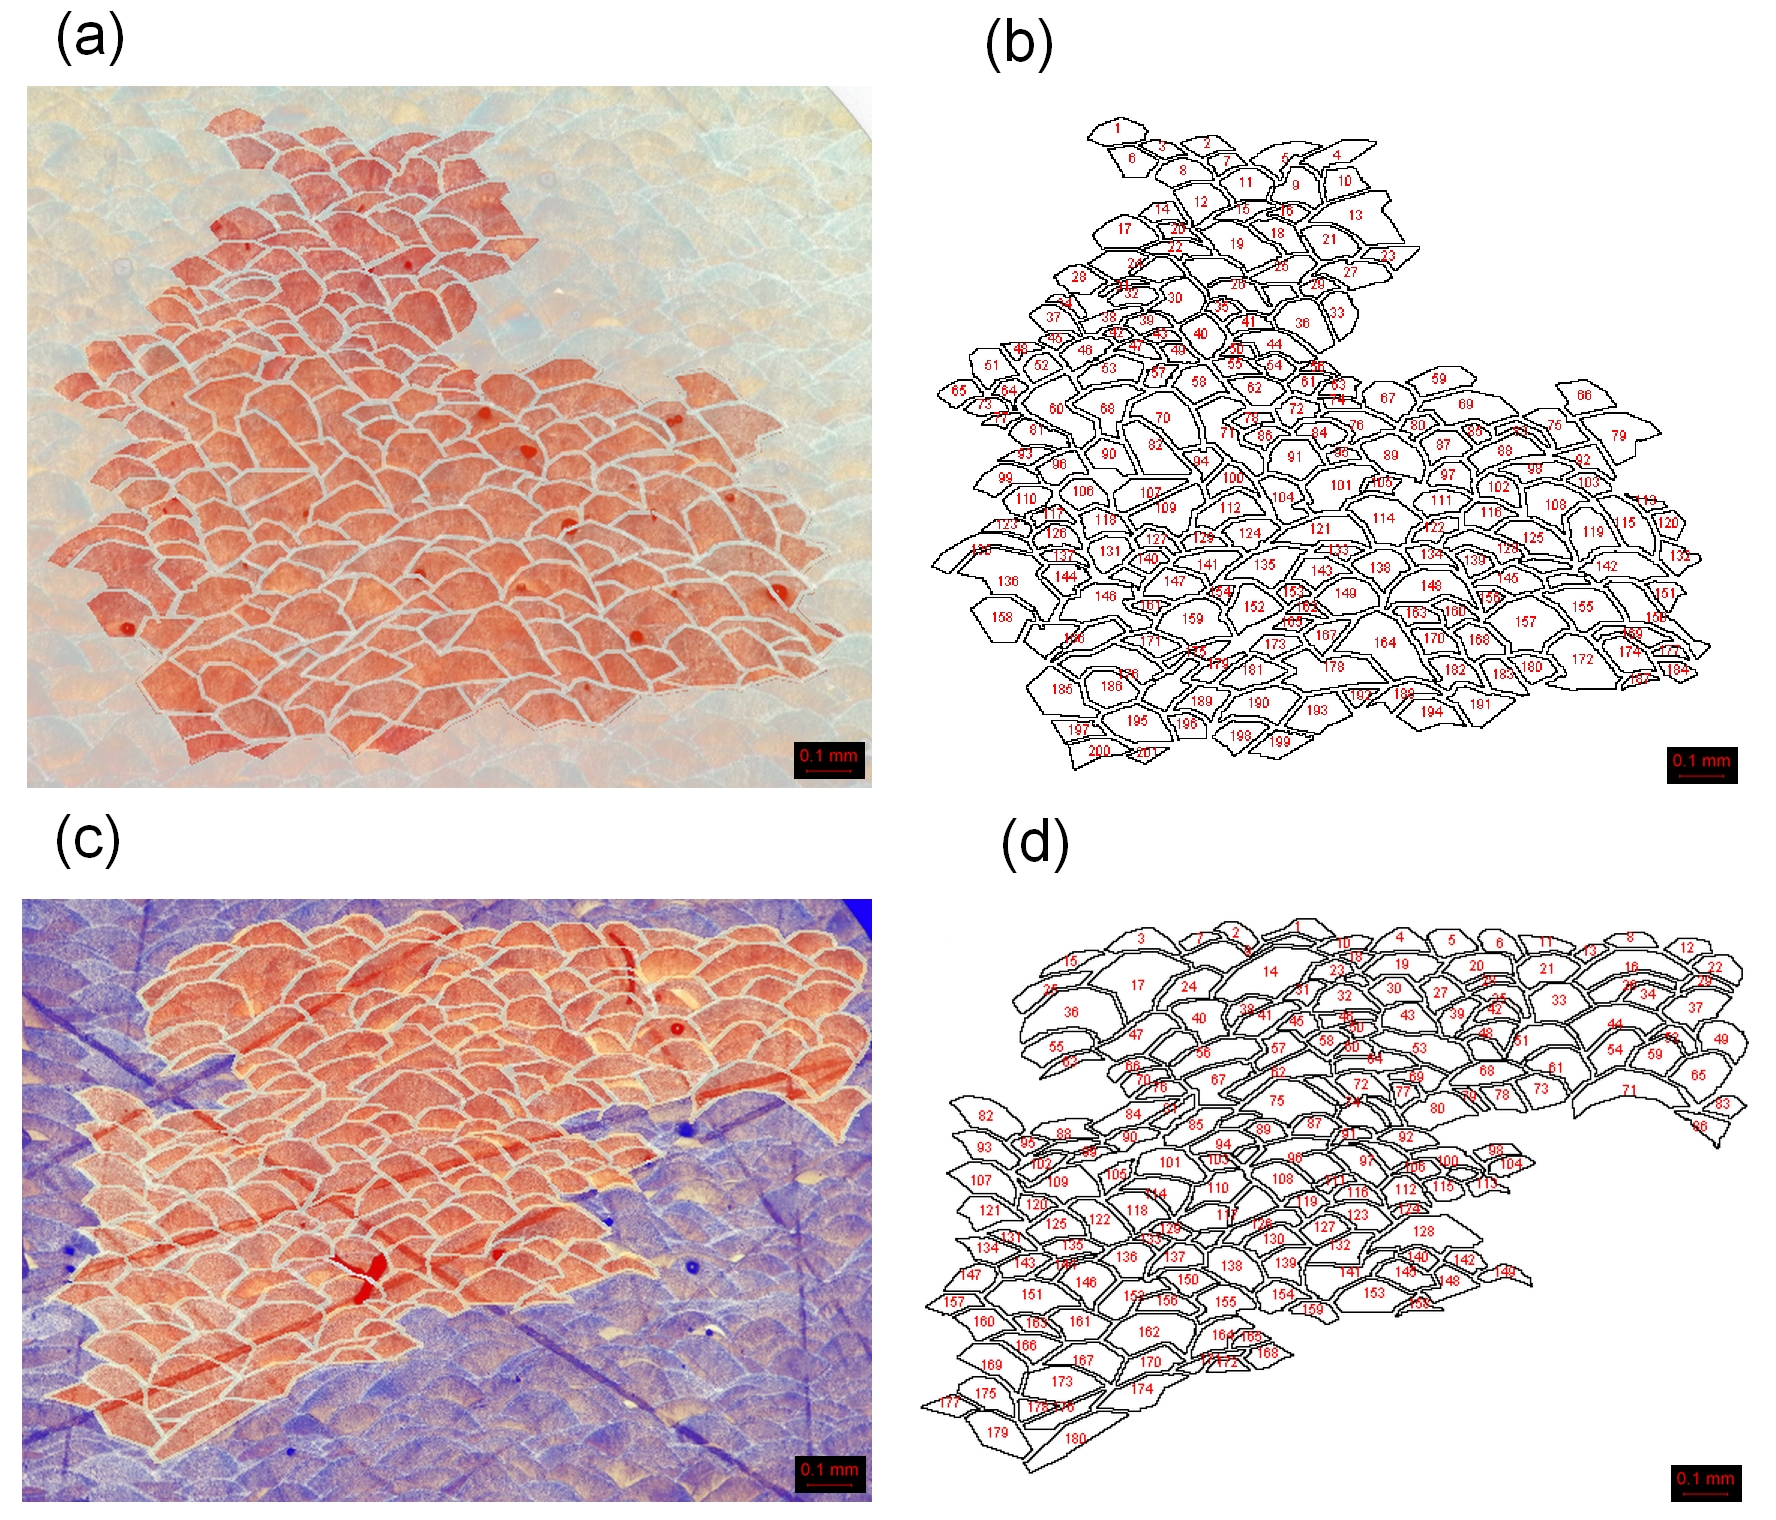
\includegraphics[scale=0.12]{Images/B1}}
\decoRule
\caption[Screen captures of (a) melt pools subdivision from a picture of specimen "8a" (b) \textit{ImageJ} partitioning from the same picture of specimen "8a" (c) melt pools subdivision from a picture of specimen "8b" (d) \textit{ImageJ} partitioning from the same picture of specimen "8b"]{Screen captures of (a) melt pools subdivision from a picture of specimen "8a" (b) \textit{ImageJ} partitioning from the same picture of specimen "8a" (c) melt pools subdivision from a picture of specimen "8b" (d) \textit{ImageJ} partitioning from the same picture of specimen "8b"}
\label{fig:B1}
\end{figure} 

In both cases, the area of every zone was computed. Melt pools areas histograms are displayed on figure \ref{fig:HistB1}. Even though the mean areas are nearly the same, the distributions are quite different (see table  \ref{tab:tracMAB}). The standard deviation for sample "8b" is approximately 50[\%] bigger than for "8a" one. The corresponding picture contains significantly more melt pools with small areas (<200 [$\mu m^2$]) and large ones (>1000 [$\mu m^2$]). \\

\begin{figure}[ht]
\centering
\centerline{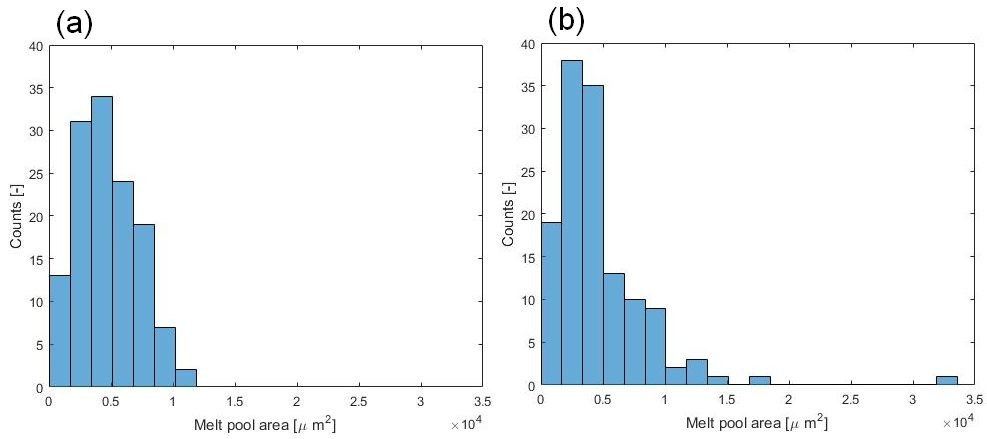
\includegraphics[scale=0.7]{Images/HistB1}}
\decoRule
\caption[Histograms of melt pools areas occurrences from \textit{ImageJ} partitioning of (a) sample "8a"  b) sample "8b"]{Histograms of melt pools areas occurrences from \textit{ImageJ} partitioning of (a) sample "8a"  b) sample "8b"}
\label{fig:HistB1}
\end{figure} 

 \begin{center}
\begin{table}[ht]
\noindent\makebox[\textwidth]{\begin{tabular}{|c |c |c|}
    \hline
     Sample & Mean area [$\mu m^2$] & SD [$\mu m^2$] \\

\hline
\hline   
    "8a" & 4.6629 $10^3$ & 2.3625 $10^3$  \\
    "8b" & 4.6597 $10^3$ & 3.9285 $10^3$  \\
    \hline
\end{tabular}}

\caption[Summary of the melt pools areas distributions for samples "8a" and "8b"]{Summary of the melt pools areas distributions for samples "8a" and "8b"}
\label{tab:tracMAB}
\end{table}
 \end{center}

\subsection{Homogeneity along the z direction}
As said in section \ref{MMFPP}, all tensile specimens were fabricated vertically. Their height is significantly greater than the other samples'; respectively 6 [cm], and 1 [cm] or less. It was chosen to cut up specimen X200-180417-25 into slices to measure if the density and hardness were homogeneous along the Z direction in the material. The surfaces analysed were named according to their original Z position in the specimen with either "B", "C1" , "C2", "C3" or "T" (for bottom, center and top) and to the test done with a letter "D" or "H"  (for density and hardness). The denomination is summarised in figure \ref{fig:saus}.\\

\begin{figure}[ht]
\centering
\centerline{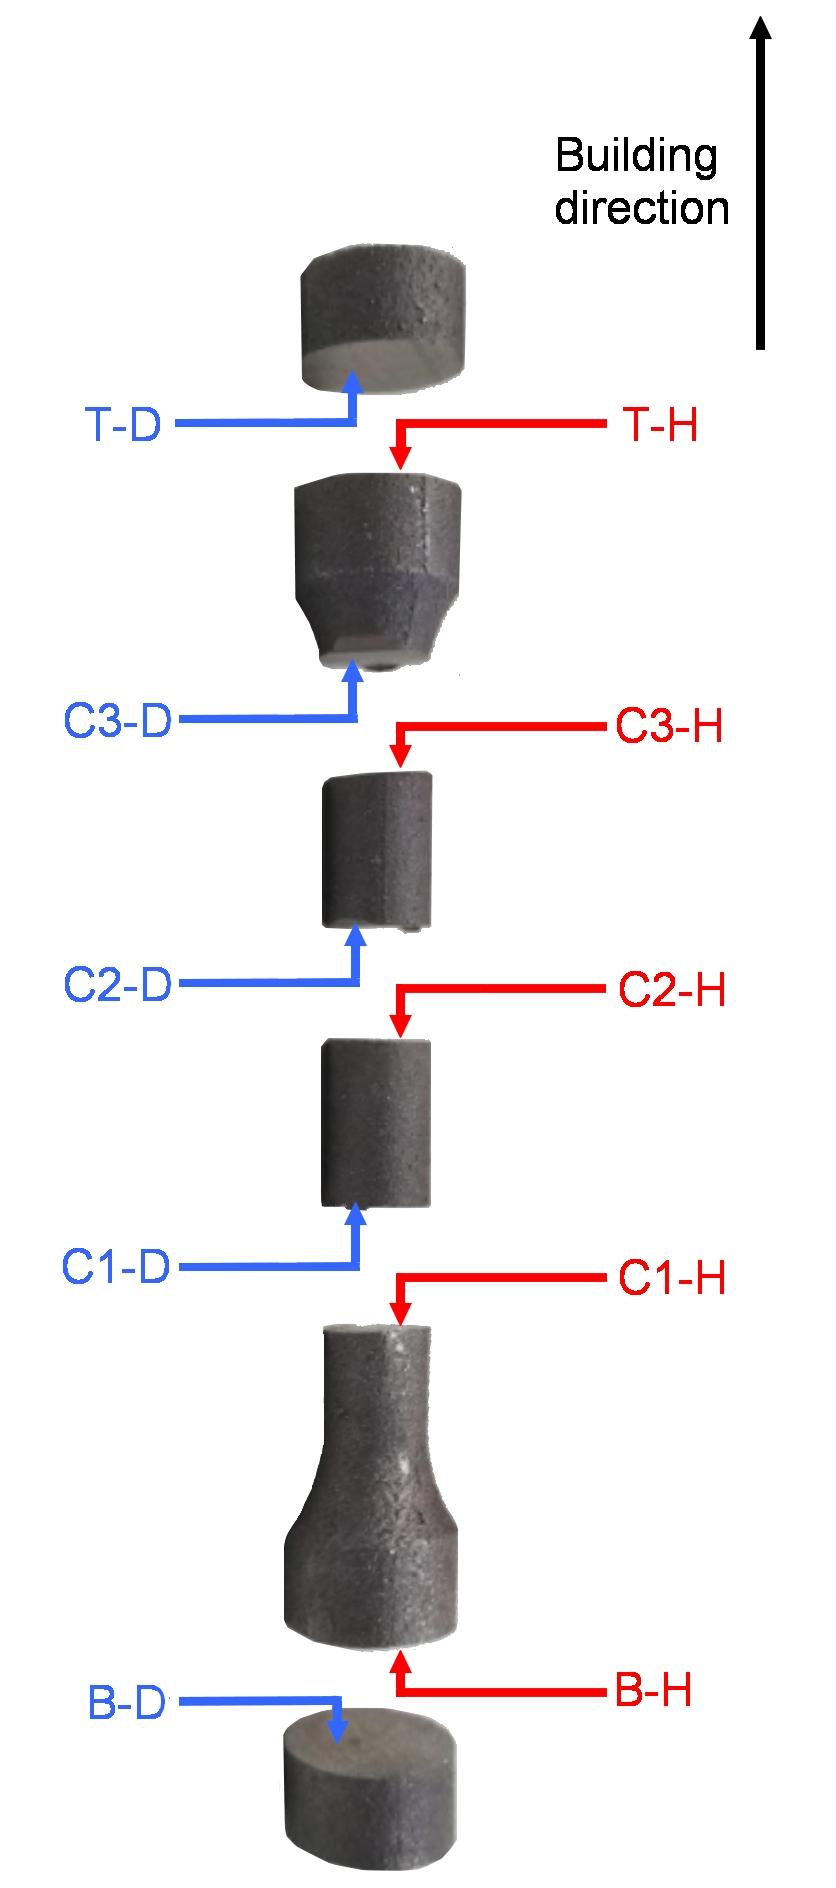
\includegraphics[scale=0.23]{Images/Saus}}
\decoRule
\caption[Specimen X200-180417-25 sub-parts and surfaces denomination]{Specimen X200-180417-25 sub-parts and surfaces denomination.}
\label{fig:saus}
\end{figure}

Results are shown in figure \ref{fig:HD-180417}. No general trend could be observed with respect to hardness. The measured values are high and closely packed except for the "B" surface, which exhibited a significantly lower hardness. Density values are all equal or above 99.75 [\%]. The values at the center of the sample were slightly lower to the extremities'. A summary of the results is displayed in table \ref{tab:25}.

 \begin{center}
	\begin{table}[ht]
		\begin{tabular}{|c|c |c |c| c|}
			\hline
			Property& Average value & Minimum & Maximum & Standard deviation \\
			\hline 
			\hline   
			Relative density [\%] & 99.80 & 99.75 & 99.87 & 0.05\\
			Hardness [HV] &138.0 &132.2 &141.7&3.5\\
			\hline
		\end{tabular}

		\caption[Relative density and hardness results summary for specimen X200-180417-25 surfaces]{Relative density and hardness results summary for specimen X200-180417-25 surfaces}
		\label{tab:25}
	\end{table}
\end{center}


\begin{figure}[ht]
\centering
\centerline{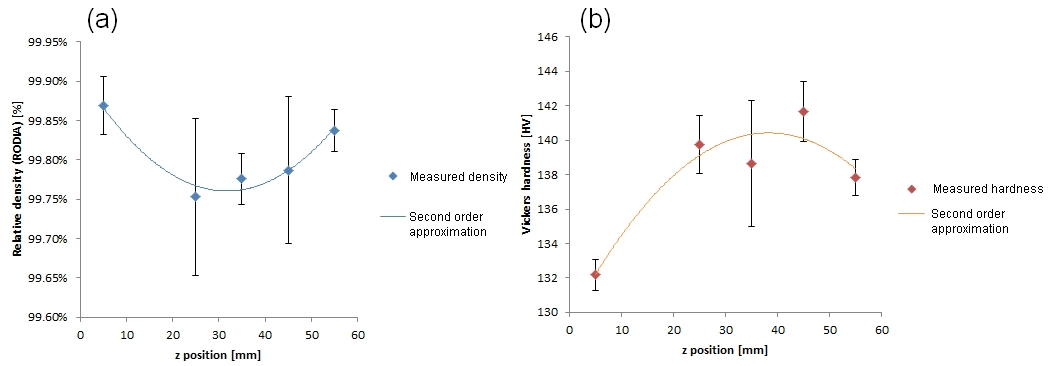
\includegraphics[scale=0.72]{Images/SausHD}}
\decoRule
\caption[Scatter plots of the results for specimen X200-180417-25 surfaces as a function of the vertical position: (a) RODIA based relative density (b) Vickers hardness]{Scatter plots of the results for specimen X200-180417-25 surfaces as a function of the vertical position: (a) RODIA based relative density (b) Vickers hardness}
\label{fig:HD-180417}
\end{figure} 


\section{In-depth characterisation of the as-built samples} 
\label{RCABS}

\subsection{Mechanical properties}

The average tensile properties of the six tested as-built specimens are displayed in table \ref{tab:tracMAB}. Detailed information may be consulted in appendice \ref{AppendixAbis}. All data was computed based on the procedures of section \ref{MMTT}. A typical curve is shown on figure \ref{fig:trac2}.\\

 \begin{center}
\begin{table}[ht]
\noindent\makebox[\textwidth]{\begin{tabular}{|c |c |c| c|}
    \hline
     E [GPa] & $\sigma_y$ [MPa] & $\sigma_u$ [MPa] & $\epsilon_f$[\%] \\

\hline
\hline   
    64.9 $\pm 3.0$ & 266.6 $\pm 23.6$ & 381.7 $\pm 24.7$ & 2.5 $\pm 0.5$  \\

    \hline
\end{tabular}}

\caption[Average tensile mechanical properties of the as-built specimens from batch X200-180417]{Average tensile mechanical properties of the as-built specimens from batch X200-180417}
\label{tab:tracMAB}
\end{table}
 \end{center}
 
 \begin{figure}[ht]
\centering
\centerline{\includegraphics[scale=0.68]{Images/trac2}}
\decoRule
\caption[Engineering tensile stress-strain curve for specimen X200-180417-2]{Engineering tensile stress-strain curve for specimen X200-180417-2}
\label{fig:trac2}
\end{figure} 
 
One specimen built with no contour scanning strategy was tested. Its tensile behaviour was observed to be very similar to the other samples. No distinction shall thus be made between the two types in what follows. Stress-strain curve for specimen X200-180417-1 was non-linear before the plasticity regime started. This is due to slippage in the grips. The obtained Young's modulus for the test was thus not taken into account for the computation of the average value.\\

No necking phenomena was observed among all tensile tests for AB samples. The Considere criterion was used for the detection of plastic instability. It states that necking starts at $\frac{d\sigma_{true}}{d\epsilon_{true}}=\sigma$, which is equivalent to $\frac{d\sigma_{eng}}{d\epsilon_{eng}}=0$. The latter condition was not satisfied for any AB engineering stress-strain curve.\\

\subsection{Microstructure}

[Optique:Tableau d'Olivier complété avec images à l'endroit et avec échelles] 

Optique: Porosité en grande majorité aux interfaces des bains de fusion. Grandes zones non fondues (?).

SEM: microstructure à mettre en // avec les faciès de rupture. Zones grossières séparées des zones fines

Faciès: 
Lisse: Porosité, clivage ou manque de fusion. Manque de fusion reconnaissable via dendrites interrompues, boules de poudre et surface non collée à la suivante.\\

As-built samples present as expected an inhomogeneous microstructure divided into scan tracks. The 3 different zones forming a scan track can be observed in Fig. \ref{fig:ms_zones}.\\

\begin{figure}[ht]
	\centering
	\centerline{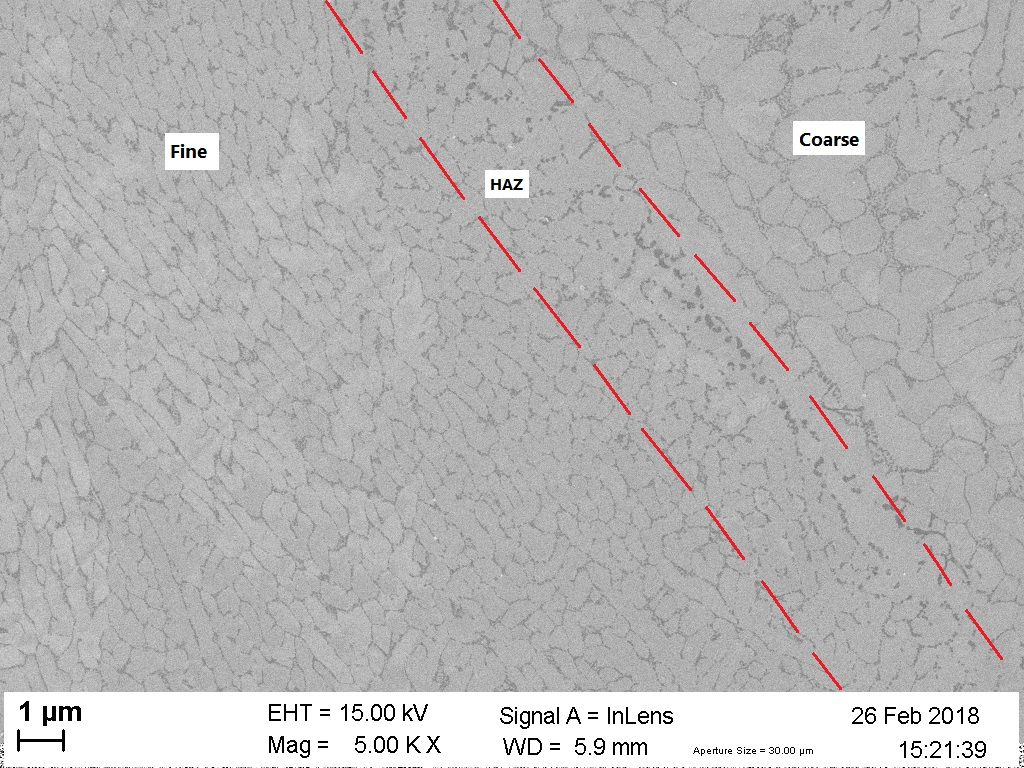
\includegraphics[scale=0.50]{Images/SEM-7b-18.png}}
	\decoRule
	\caption[Microstructure of an as-built sample with the 3 different zones visible, indicating the edge of the melting pool]{Microstructure of an as-built sample with the 3 different zones visible, indicating the edge of the melting pool.}
	\label{fig:ms_zones}
\end{figure}

The presence of these 3 zones makes it impossible to give a single representative value to represent the size of the whole microstructure. The equiaxed cells from the fine zone core have a mean size below 1 $\mu$m, lying generally between 0.4 and 0.7 $\mu$m. The coarse zone at the melt pool boundary presents slightly larger cells with a size between 0.8 and 1.2 $\mu$m.

\subsubsection{Damage and fractography}

 Some of the ruptured tensile samples had their fracture surface directly observed via SEM, as shown in Fig. \ref{fig:ms_ab_frac}. Near the edge are present some "step-like" structures, visible on Fig. \ref{fig:ms_ab_frac2}. their width is ranging from 70 to 110 $\mu$m, which is similar to the hatch space of the SLM process. It would suggest that failure takes place at the boundary between melt pools, where the microstructure is coarser, as discussed by Aboulkhair et al. \cite{Rosenthal17}.\\

\begin{figure}[ht]
	\centering
	\centerline{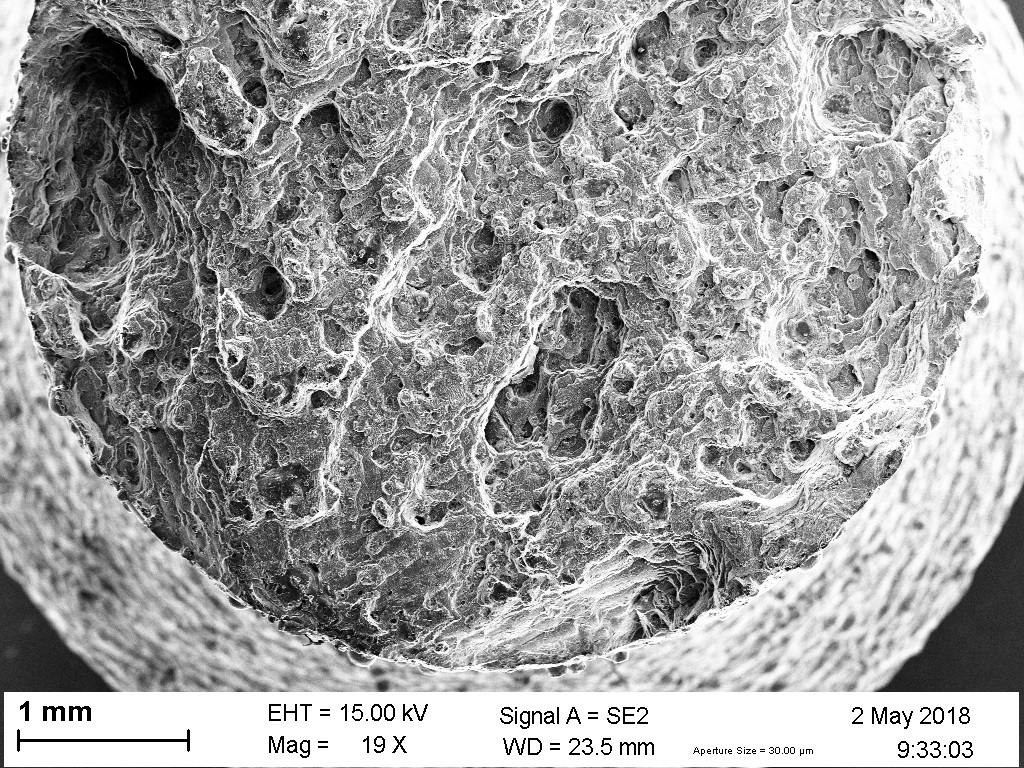
\includegraphics[scale=0.50]{Images/frac-01-04.png}}
	\decoRule
	\caption[Fractograph of an as-built tensile sample]{Fractograph of an as-built tensile sample.}
	\label{fig:ms_ab_frac}
\end{figure}

\begin{figure}[ht]
	\centering
	\centerline{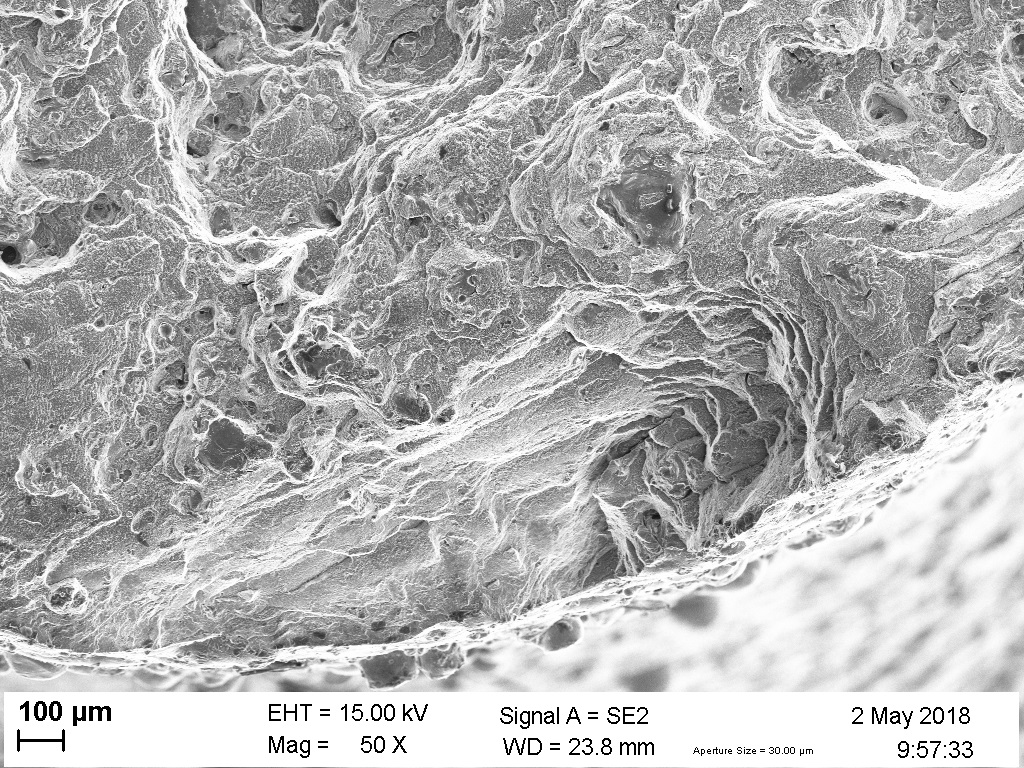
\includegraphics[scale=0.35]{Images/frac-01-12.jpg}}
	\decoRule
	\caption["Step-like" structure appearing on the edge of the as-built tensile sample]{"Step-like" structure appearing on the edge of the as-built tensile sample.}
	\label{fig:ms_ab_frac2}
\end{figure}

Taking a closer look reveals on Fig. \ref{fig:ms_ab_frac3} the presence of dimples on an important fraction of the surface. Their size seems to vary mainly between 0.3 and 0.7$\mu$m. But smoother areas are also visible on the surface (see Fig. \ref{fig:ms_ab_frac4}). The presence of unmelted powder particles indicates that the area has known a lack of fusion. It causes bad cohesion between the consecutive layers and represents an important defect, able to initiate premature failure.\\

\begin{figure}[ht]
	\centering
	\centerline{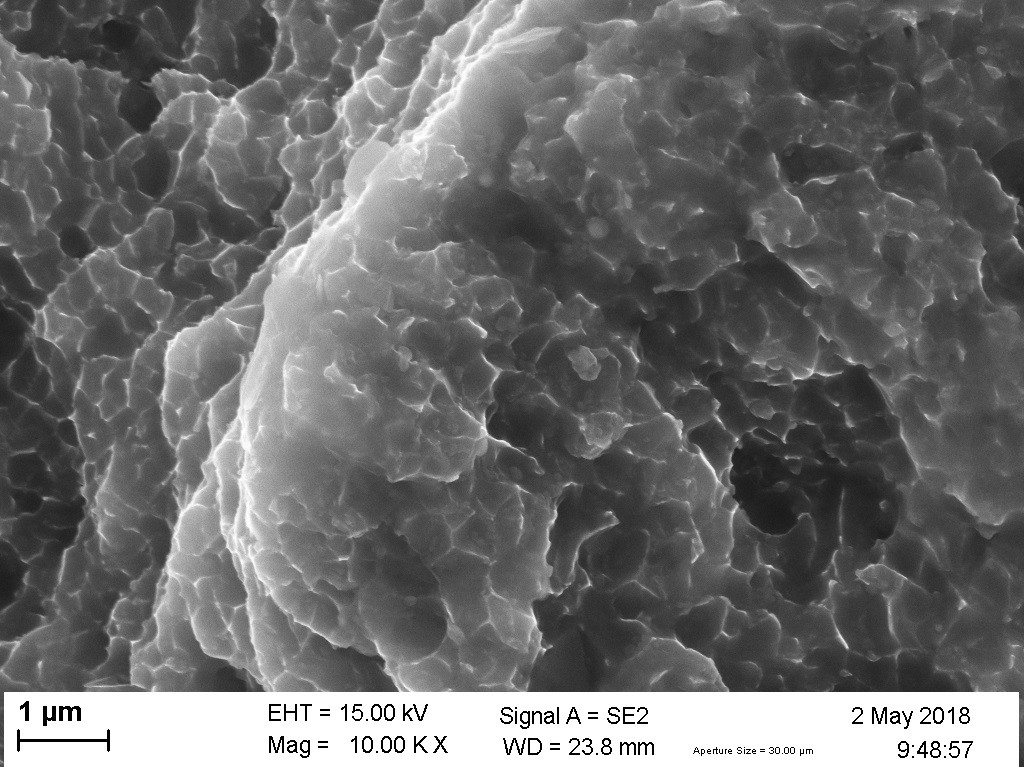
\includegraphics[scale=0.35]{Images/frac-01-09.jpg}}
	\decoRule
	\caption[Close-up shot on the ductile dimples of the as-built fracture surface]{Close-up shot on the ductile dimples of the as-built fracture surface.}
	\label{fig:ms_ab_frac3}
\end{figure}

\begin{figure}[ht]
	\centering
	\centerline{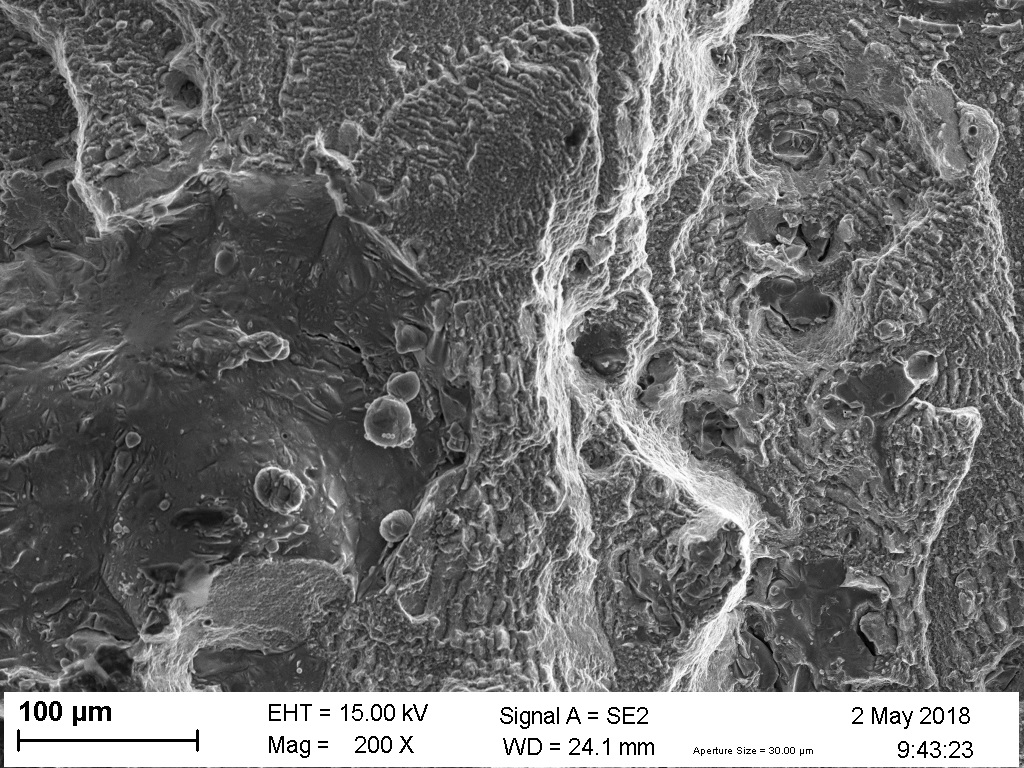
\includegraphics[scale=0.35]{Images/frac-01-07.jpg}}
	\decoRule
	\caption[View of the smooth fracture surface (on the left). A couple unmelted powder particles are visible]{View of the smooth fracture surface (on the left). A couple unmelted powder particles are visible.}
	\label{fig:ms_ab_frac4}
\end{figure}

Microstructure damage after fracture was also observed via SEM. An example is available in Fig. \ref{fig:ms_ab_dmg}. The cells are strongly oriented in the loading direction. Their average size in this direction is 1.2$\mu$m, while it is only 0.6 $\mu$m in the perpendicular direction.\\

\begin{figure}[ht]
	\centering
	\centerline{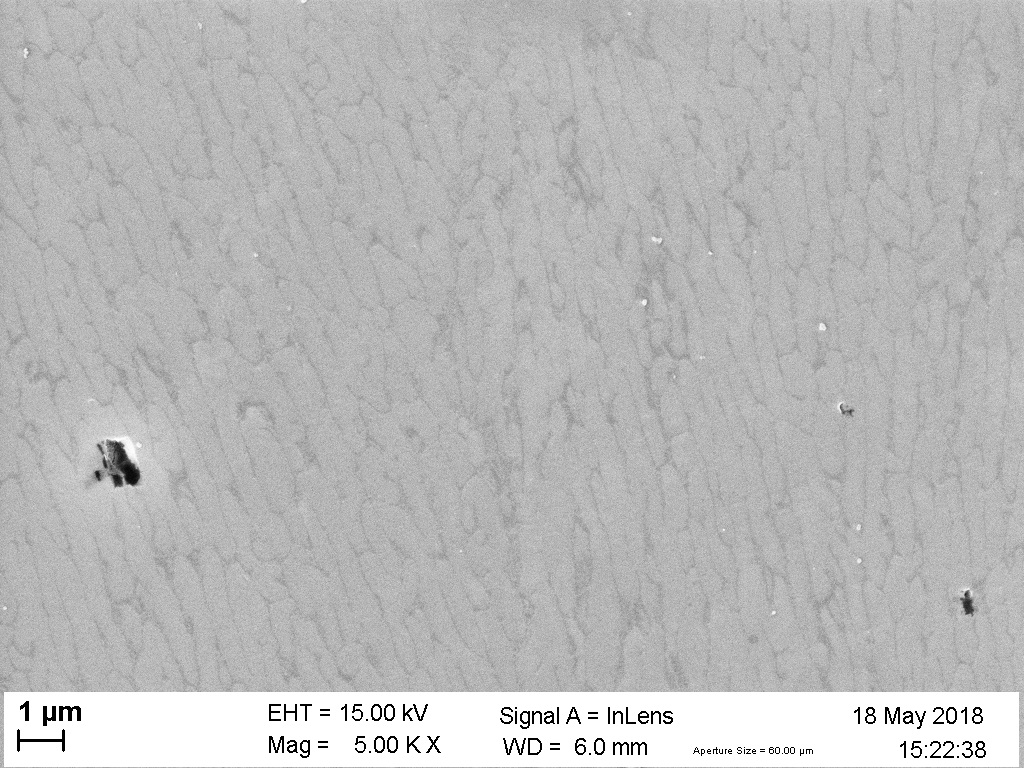
\includegraphics[scale=0.35]{Images/dmg-01-03.jpg}}
	\decoRule
	\caption[Microstructure damage after rupture. The picture is taken roughly 40 $\mu$m below the fracture surface. The loading direction is vertical]{[Microstructure damage after rupture. The picture is taken roughly 40 $\mu$m below the fracture surface. The loading direction is vertical.}
	\label{fig:ms_ab_dmg}
\end{figure}

\section{In-depth characterisation of the heat-treated samples}
\label{RCHTS}

\subsection{Density}
The density of most of the heat treated cubes of dimensions 5 x 5 x 5 [$mm^3$] was measured through RODIA (see table \ref{tab:densTT}). The 95\% CI are also indicated.\\

 \begin{center}
\begin{table}[ht]
\noindent\makebox[\textwidth]{\begin{tabular}{|c|c|c|}
    \hline
     Temperature [$^\circ C$] & Holding time [min] & $\rho_{rel}$ [\%]\\

\hline
\hline   
   150 & 120 & 99.83 $\pm 0.02$\\
   200 & 120 & 99.82 $\pm 0.04$\\
   225 & 120 & 99.88 $\pm 0.01$\\
   250 & 120 & 99.77 $\pm 0.04$\\
   300 & 5 & 99.85 $\pm 0.02$\\
   300 & 120 & 99.77 $\pm 0.04$\\

    \hline
\end{tabular}}

\caption[RODIA relative density results for the heat treated cubes]{RODIA relative density results for the heat treated cubes}
\label{tab:densTT}
\end{table}
 \end{center}

All samples came from the same batch (X200-180220) except for TT225-2 one which originated from batch X200-180319. The samples from the latter had significantly better properties than the other batches'. This particular specimen should thus not be compared to the others. The other samples treated during two hours show a slight decrease of $\rho_{rel}$ as a function of the temperature. The relative density measured for TT300-5m, that was heated for a short duration, is superior to the other's. Nevertheless, caution should be exercised here since the measured differences are small (inferior to a tenth of percent). 

\subsection{Hardness}

Heat-treated samples were subjected to hardness tests identical to those performed on as-built cubes. Their result is given in Fig. \ref{fig:hardness}.

\begin{figure}[ht]
	\centering
	\centerline{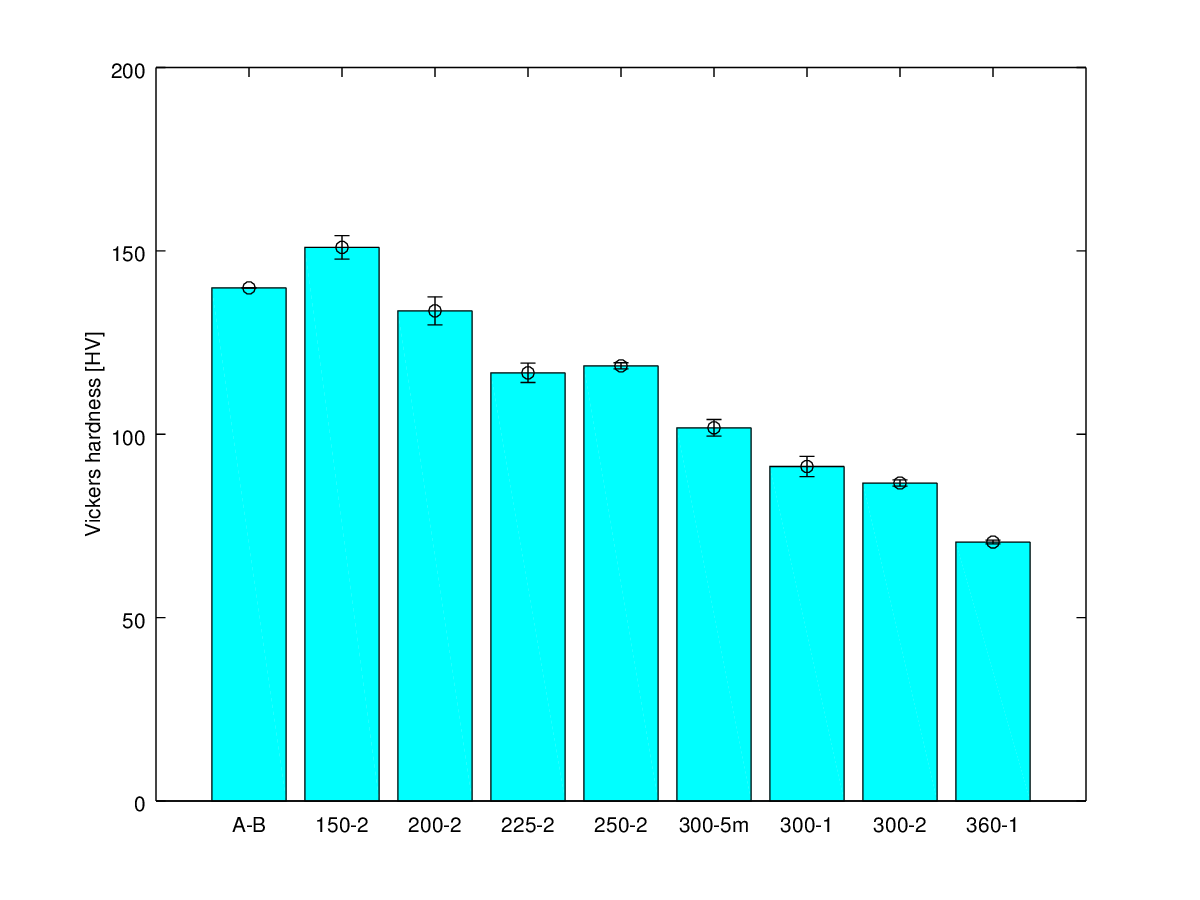
\includegraphics[scale=0.6]{Images/hardness.png}}
	\decoRule
	\caption[Comparison of the heat-treated samples hardness with the as-built.]{Comparison of the heat-treated samples hardness with the as-built.}
	\label{fig:hardness}
\end{figure}


\subsection{Mechanical properties}

Tensile tests were made on heat treated specimens. All samples had undergone a HT during 2h, at either 150$^\circ C$, 200$^\circ C$, 250 $^\circ C$ or 300 $^\circ C$. Three samples were tested for each HT except for the one at 250 $^\circ C$ (only two samples). One specimen heated at 150$^\circ C$ was fabricated with no contour scanning strategy. The results are gathered in \ref{AppendixB}. Typical curves for each heat treatment are displayed in figure \ref{fig:tracTT}. The average tensile properties for each HT are shown in table \ref{tab:tracMHT}. All samples heated at 250$^\circ C$ and 300$^\circ C$ went through necking in the sense of Considère criterion. Their $\epsilon_{f,true}$ was computed thanks to a profile projector. \\

 \begin{center}
\begin{table}[ht]
\noindent\makebox[\textwidth]{\begin{tabular}{|c|c |c |c| c|c|}
    \hline
     HT & E [GPa] & $\sigma_y$ [MPa] & $\sigma_u$ [MPa] & $\epsilon_{f,eng}$[\%] & $\epsilon_{f,true}$ [\%] \\

\hline
\hline   
   150$^\circ$C (2h) & 68.4 $\pm 1.9$ & 288.2 $\pm 1.4$ & 441.7 $\pm 5.5$ & 3.1 $\pm 0.4$&-  \\
    200$^\circ$C (2h) &  72.1 $\pm 0.4$ & 245.4 $\pm 0.6$ & 382.0 $\pm 11.4$ & 2.6 $\pm 0.2$ &- \\
     250$^\circ$C (2h) &  70.6 $\pm 1.0$ & 235.1 $\pm 7.4$ & 340.9 $\pm 12.2$ &8.8 $\pm 0.2$ & 16.5 $\pm 0.1$  \\
      300$^\circ$C (2h) &  68.9 $\pm 0.6$ & 170.7 $\pm 1.7$ & 252.9 $\pm 10.4$ &13.6 $\pm 0.5$ & 29.7 $\pm 0.1$  \\

    \hline
\end{tabular}}

\caption[Average tensile mechanical properties of the heat-treated specimens from batch X200-180417]{Average tensile mechanical properties of the heat-treated specimens from batch X200-180417}
\label{tab:tracMHT}
\end{table}
 \end{center}

\begin{figure}[ht]
\centering
\centerline{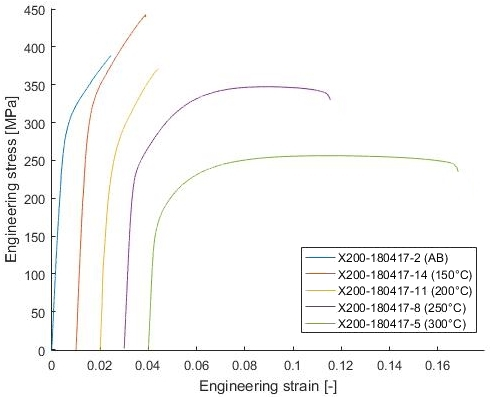
\includegraphics[scale=0.7]{Images/TracTT}}
\decoRule
\caption[Engineering stress-strain curves of heat treated tensile specimens of batch X200-180417.]{Engineering stress-strain curves of heat treated tensile specimens of batch X200-180417.}
\label{fig:tracTT}
\end{figure}


The heat treatment at 150$^\circ$ increased notably $\sigma_u$ compared to the as-built values. However, the heating at 200$^\circ$ caused virtually no change of ultimate tensile strength. None of these heat treatment caused any significant change of fracture strain. For HT at 250$^\circ$ and 300$^\circ$, the material softened significantly (with necking appearance); the higher the heating temperature, the bigger the ductility increased and the strength decreased. The Young's modulus measured for heat treated samples was significantly bigger in average 69.9 [GPa] compared to 64.9 [GPa].\\

The average $\sigma_{true}$-$\epsilon_{true}$ data was also displayed in a graphical form for better insight. The true stress and strain were approximated by the engineering ones for samples with no necking. %As the curves for a same HT do not end at the same $\epsilon_{f,true}$, the average curve could not be obtained by simply taking the mean $\sigma$ value at each $\epsilon$. This would have indeed lead to discontinuities at each fracture strain on the graph. The chosen solution was to 
A fit was made with the average properties in a Ramberg-Osgood hardening law:\\

$$\epsilon_{true}=\frac{\sigma_{true}}{E_a}+ 0.002(\frac{\sigma_{true}}{\sigma_{y,a}})^{(\frac{1}{n_a})}$$

where $n_a \simeq \epsilon_{f,true,a}$ is the strain hardening coefficient. The subscript "a" means that the average values are used. This was done with an online calculator \parencite{RO}. \\


\begin{figure}[ht]
\centering
\centerline{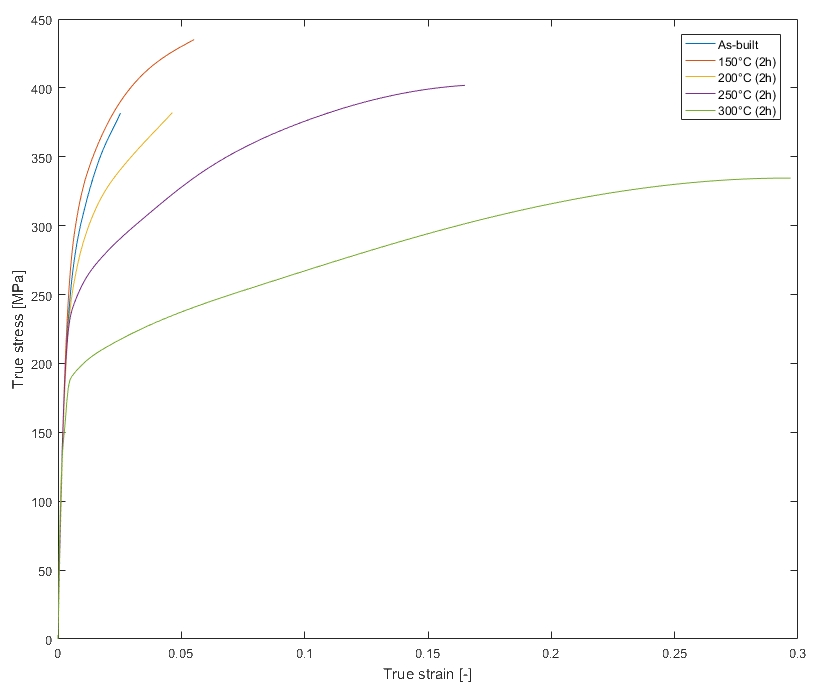
\includegraphics[scale=0.7]{Images/MeanTrac}}
\decoRule
\caption[Average stress-strain curves of the tensile specimens of batch X200-180417.]{Average stress-strain curves of the tensile specimens of batch X200-180417.}
\label{fig:MeanTrac}
\end{figure}

%\begin{table}
%\caption{The effects of treatments X and Y on the four groups studied.}
%\label{tab:treatments}
%\centering
%\begin{tabular}{l l l}
%\toprule
%\tabhead{Groups} & \tabhead{Treatment X} & \tabhead{Treatment Y} \\
%\midrule
%1 & 0.2 & 0.8\\
%2 & 0.17 & 0.7\\
%3 & 0.24 & 0.75\\
%4 & 0.68 & 0.3\\
%\bottomrule\\
%\end{tabular}
%\end{table}

\subsection{Microstructure}

As discussed in the section \ref{SOTAPT}, heat treatments can modify the fine microstructure of SLM parts.\\

\begin{figure}[ht]
	\centering
	\centerline{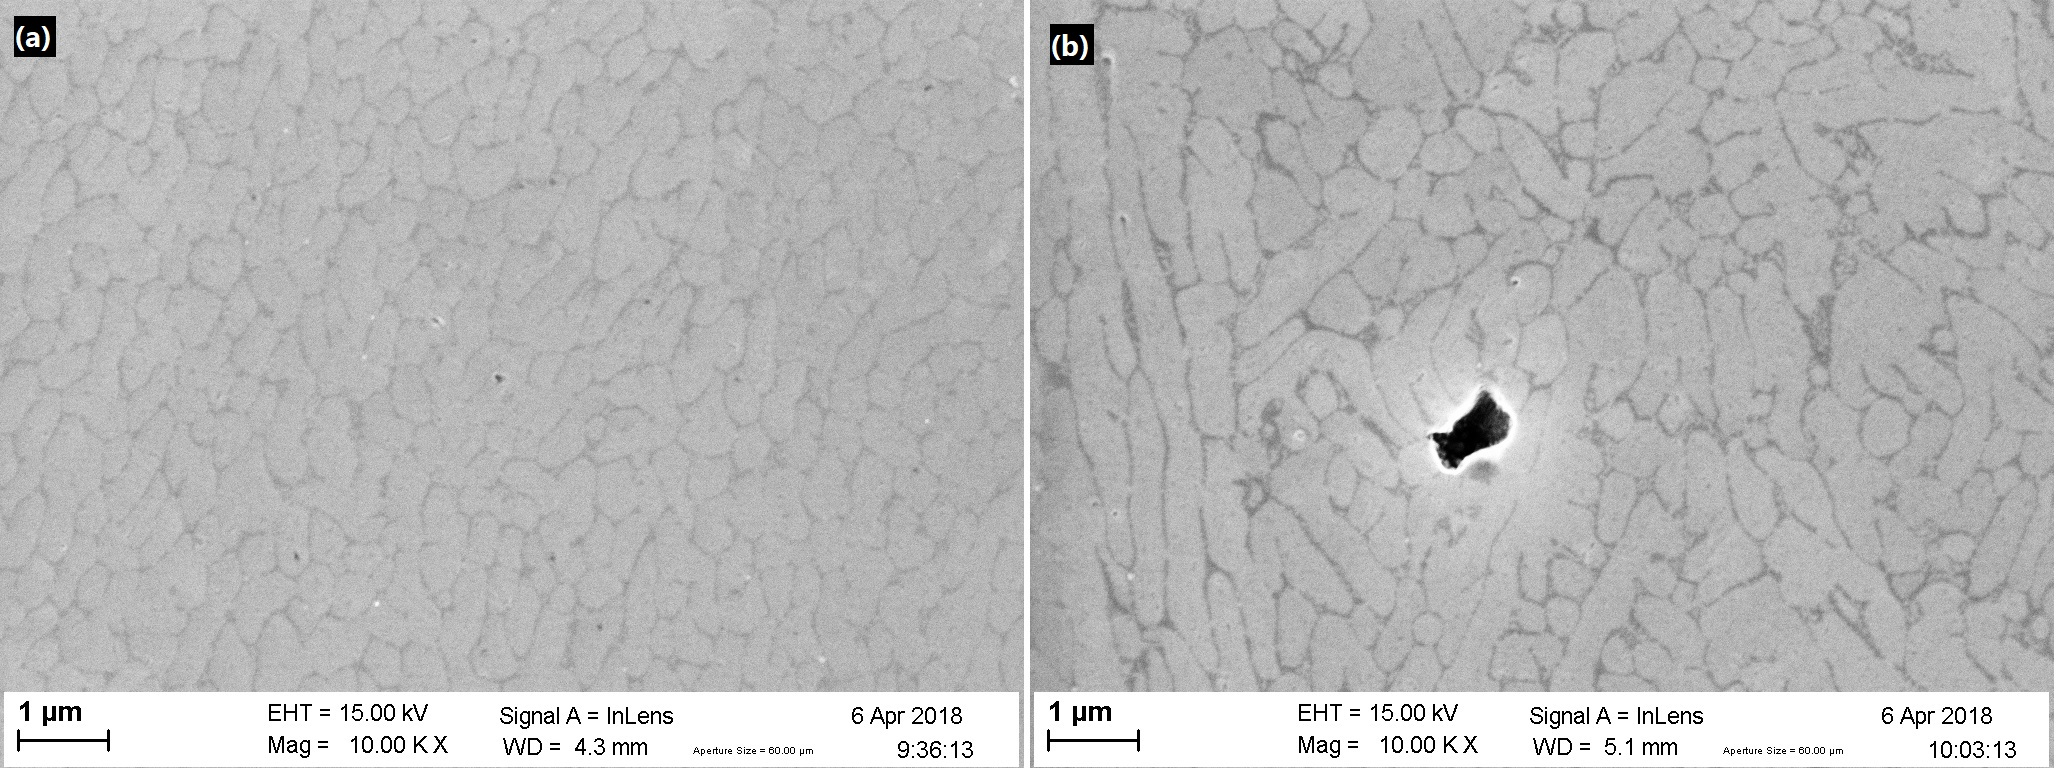
\includegraphics[scale=0.30]{Images/SEM-TT150&200-2-real}}
	\decoRule
	\caption[Microstructure of the sample heat-treated at (a) 150$^\circ$C for 2h and (b) 200$^\circ$C for 2h]{Microstructure of the sample heat-treated at (a) 150$^\circ$C for 2h and (b) 200$^\circ$C for 2h.}
	\label{fig:ms_150_200_2}
\end{figure}

Treatment at 250$^\circ$C gives an intermediate result, as shown in Fig. \ref{fig:ms_250_2}. Globularization begins to take place but most of the cellular structure remains visible. Cell size is for the most part comprised between 0.5 and 0.9 [$\mu$m], with a mean size around 0.7 [$\mu$m]. As a comparison with other samples treated at higher temperature, the particle size was calculated with ImageJ. The result was a mean particle size of 0.29 [$\mu$m]. \\

\begin{figure}[ht]
	\centering
	\centerline{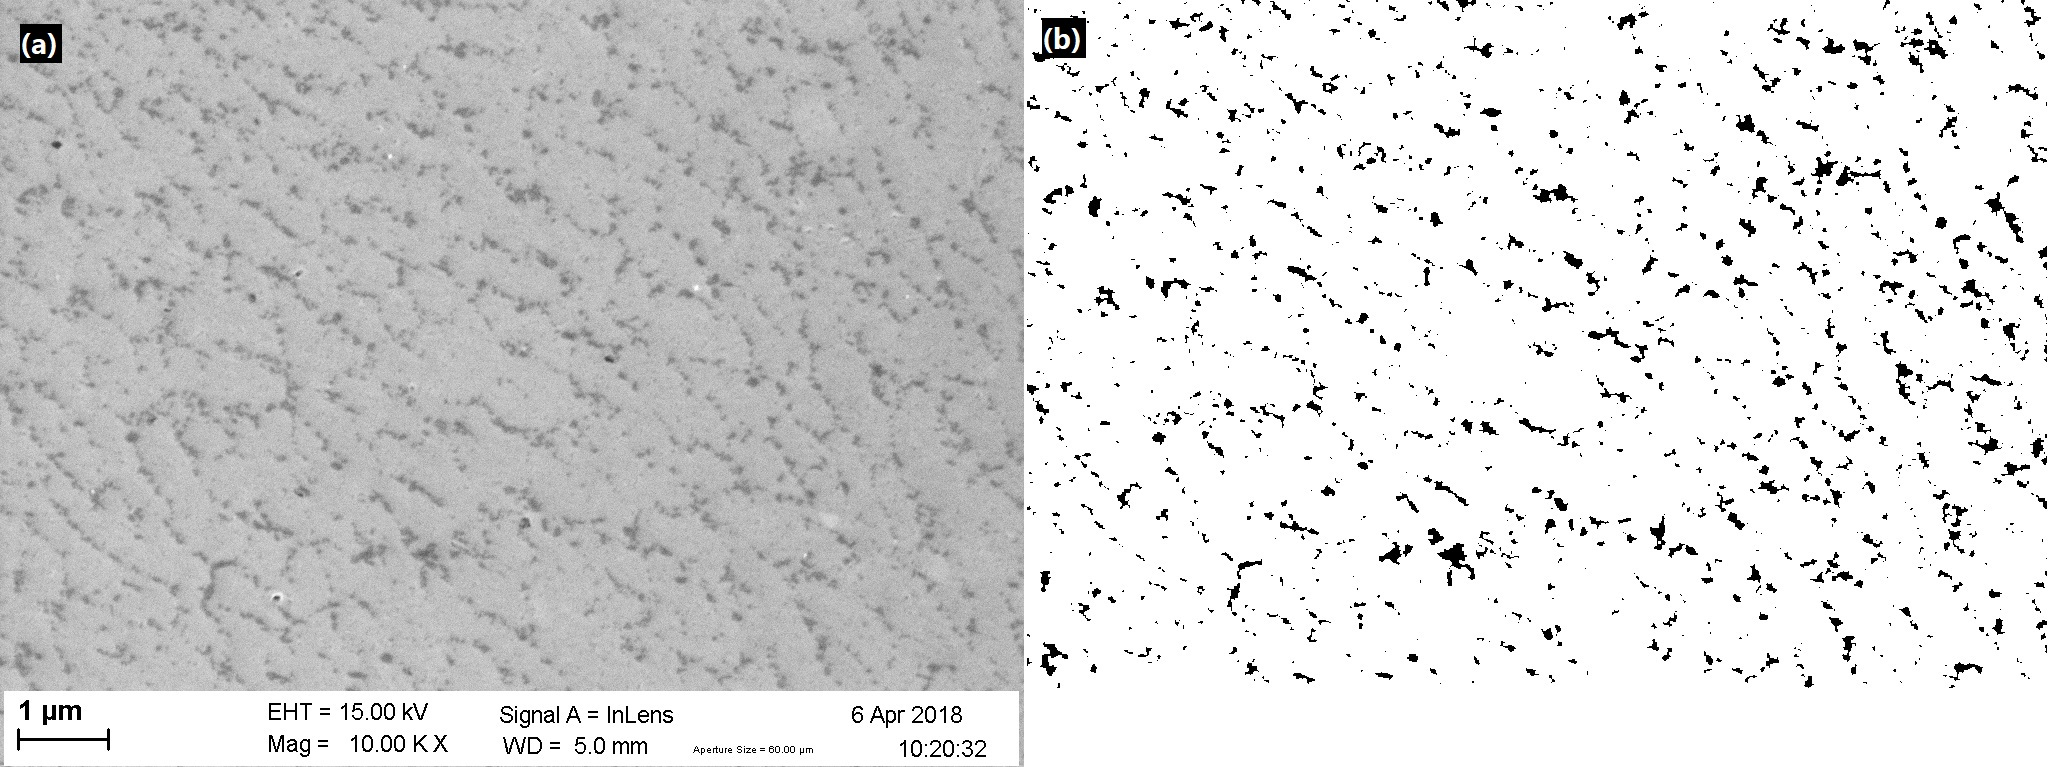
\includegraphics[scale=0.30]{Images/SEM-TT250-2-real-06.jpg}}
	\decoRule
	\caption[(a) Microstructure of the sample heat-treated at 250$^\circ$C for 2h and (b) Isolation of the Si particles via the ImageJ software]{(a) Microstructure of the sample heat-treated at 250$^\circ$C for 2h and (b) Isolation of the Si particles via the ImageJ software.}
	\label{fig:ms_250_2}
\end{figure}

Microstructure after heat treatment at 300$^\circ$C for 2 distinct holding times are available in Fig. \ref{fig:ms_300_1} and \ref{fig:ms_300_2}. The mean particle size for 1 hour and 2 hours holding time are respectively 0.22 and 0.27 [$\mu$m]. The average nearest neighbour distance are equal to 0.10 and 0.11 [$\mu$m].

\begin{figure}[ht]
	\centering
	\centerline{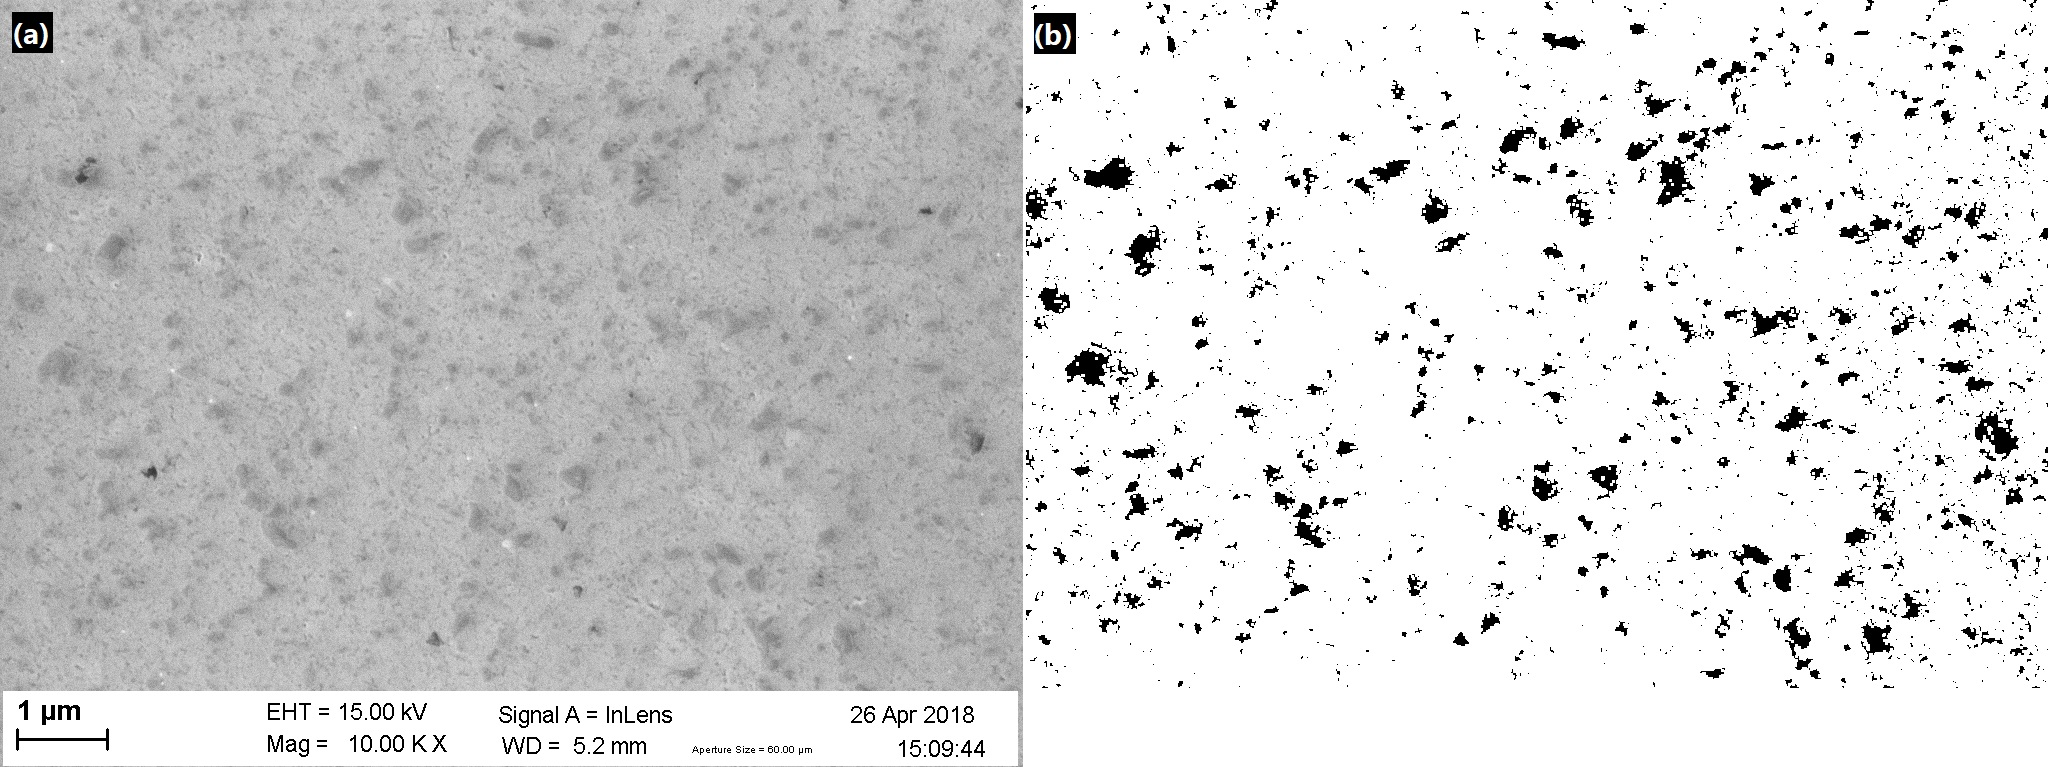
\includegraphics[scale=0.30]{Images/SEM-TT300-1-real_12.png}}
	\decoRule
	\caption[(a) Microstructure of the sample heat-treated at 300$^\circ$C for 1h and (b) Isolation of the Si particles via the ImageJ software]{(a) Microstructure of the sample heat-treated at 300$^\circ$C for 1h and (b) Isolation of the Si particles via the ImageJ software.}
	\label{fig:ms_300_1}
\end{figure}

\begin{figure}[ht]
	\centering
	\centerline{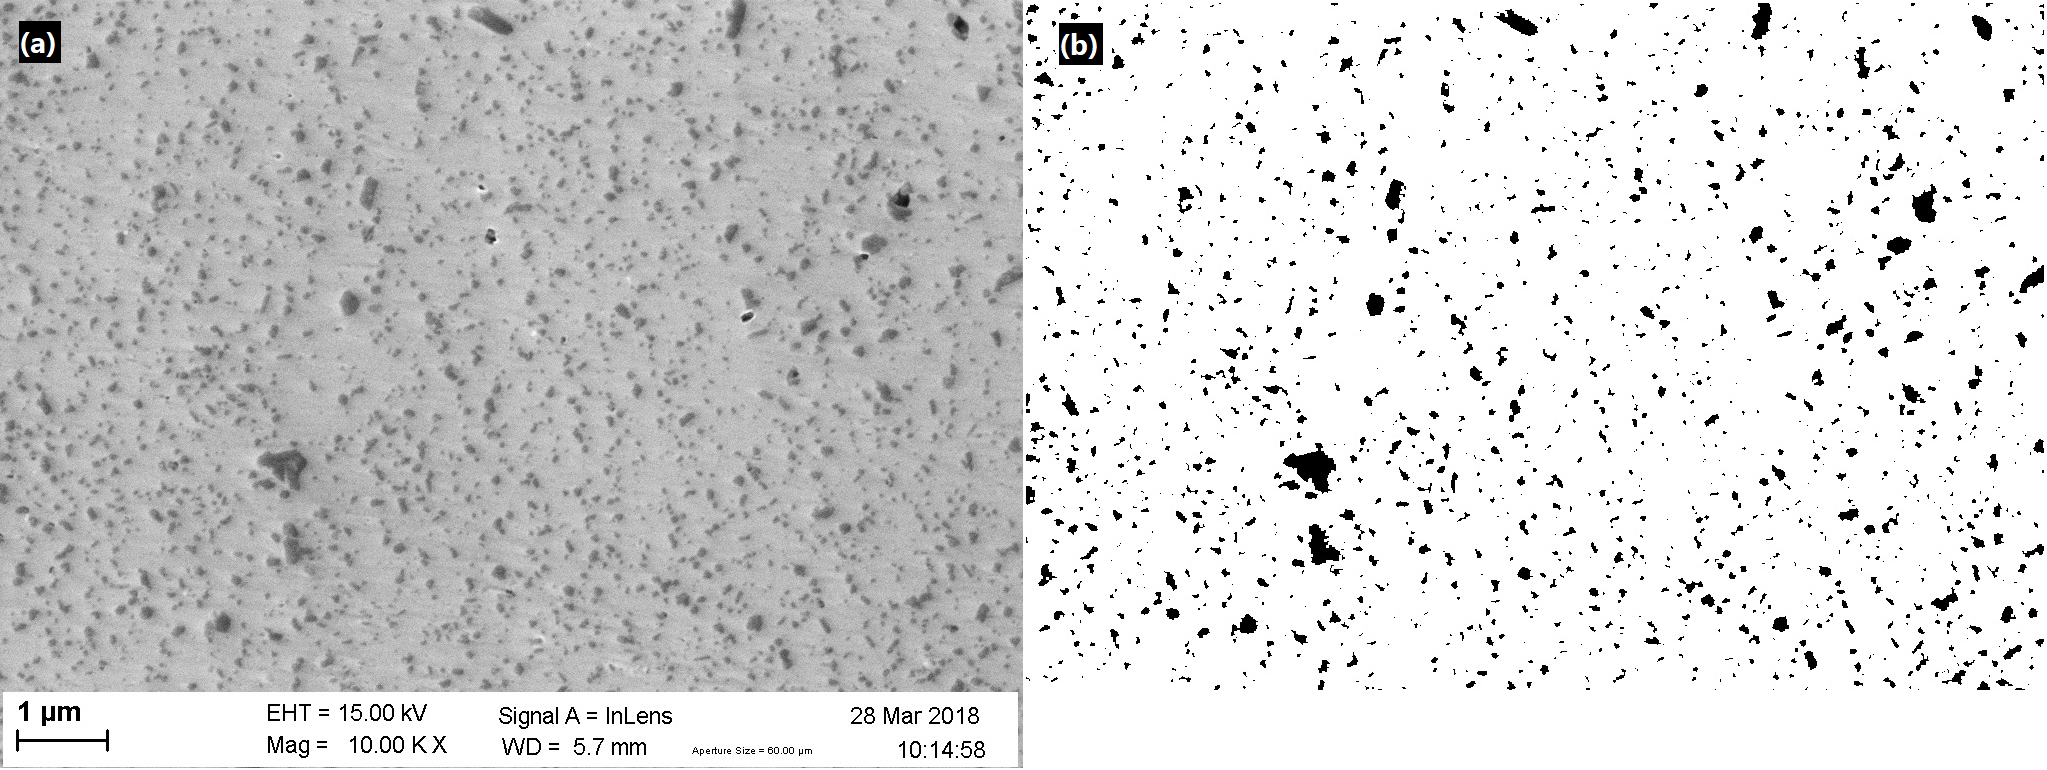
\includegraphics[scale=0.30]{Images/SEM-TT300-2-real_20.png}}
	\decoRule
	\caption[(a) Microstructure of the sample heat-treated at 300$^\circ$C for 2h and (b) Isolation of the Si particles via the ImageJ software]{(a) Microstructure of the sample heat-treated at 300$^\circ$C for 2h and (b) Isolation of the Si particles via the ImageJ software.}
	\label{fig:ms_300_2}
\end{figure}

\begin{figure}[ht]
	\centering
	\centerline{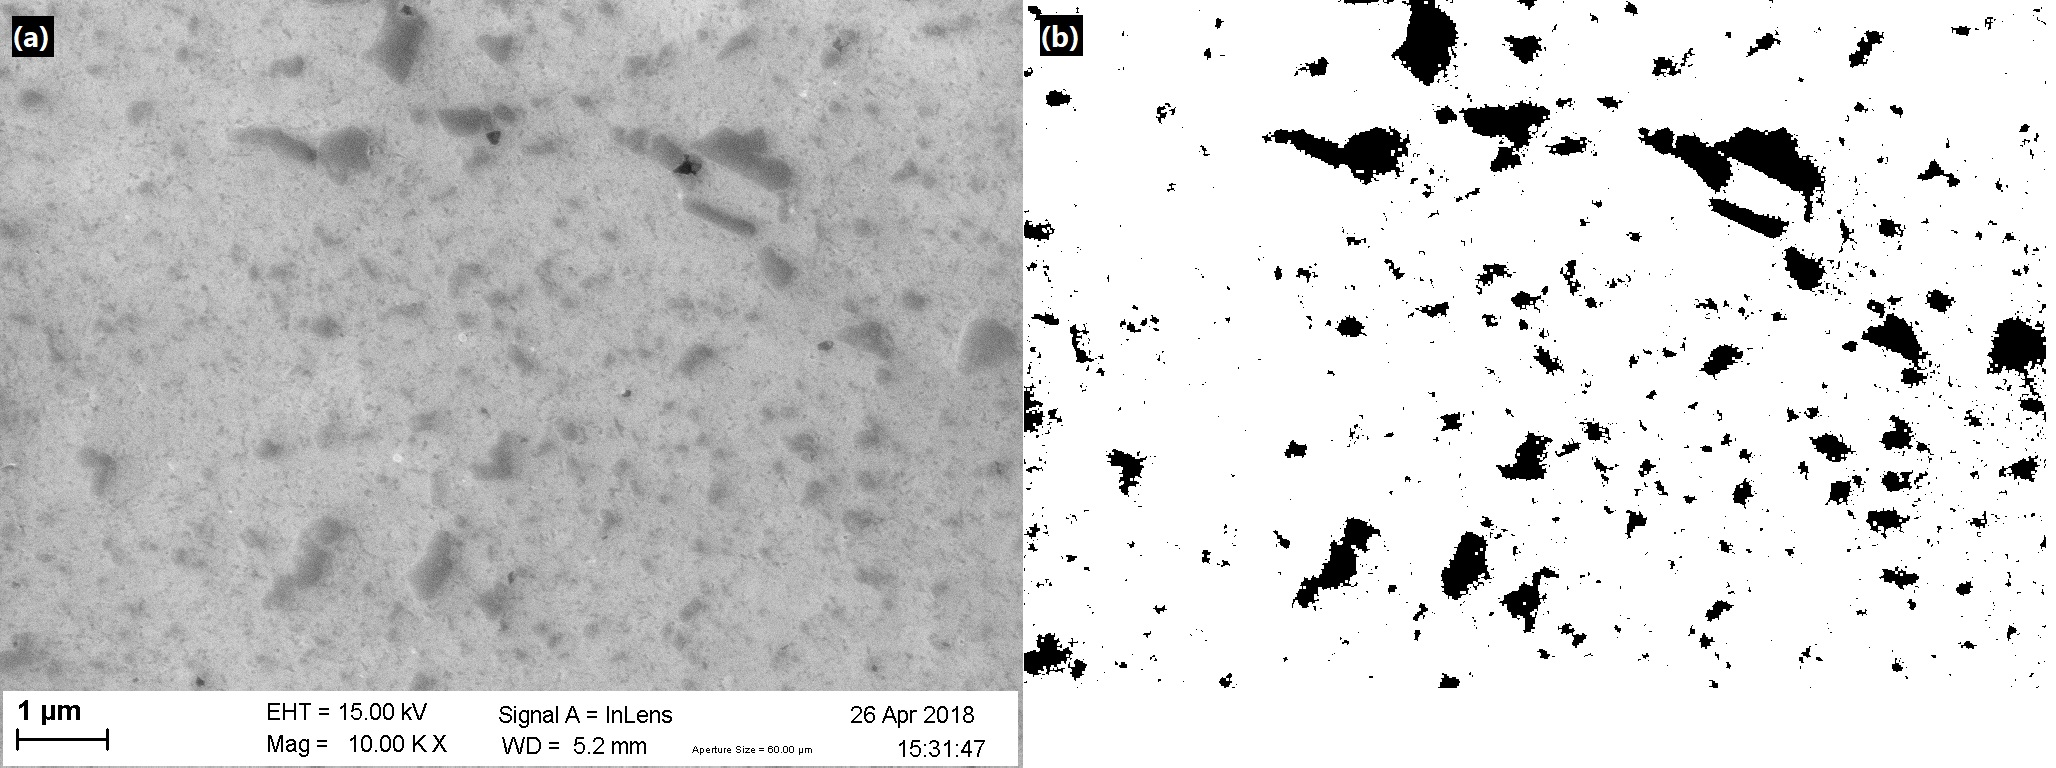
\includegraphics[scale=0.30]{Images/SEM-TT360-1-real-08.png}}
	\decoRule
	\caption[(a) Microstructure of the sample heat-treated at 360$^\circ$C for 1h and (b) Isolation of the Si particles via the ImageJ software]{(a) Microstructure of the sample heat-treated at 360$^\circ$C for 1h and (b) Isolation of the Si particles via the ImageJ software.}
	\label{fig:ms_360_1}
\end{figure}

\subsubsection{Damage and fractography}

Fracture surfaces of heat-treated samples keep several common characteristics with as-built surfaces. The parallel lines delimiting scan tracks remain visible after every annealing, up to 300$^\circ$C holding for 2h, as shown in Fig. \ref{fig:frac_04_01}. The same observation can be made for regions showing a lack a fusion, as displayed in Fig. \ref{fig:frac_04_11}.\\

Most of the surface is covered of dimples, visible on Fig. \ref{fig:frac_04_08}, with an average size of ... [$\mu$m]. A higher contrast between the dimples bottom and ridges could however indicate a larger height difference. This would mean that the ridges undergo higher plastic strain before failure.\\



\begin{figure}[ht]
	\centering
	\centerline{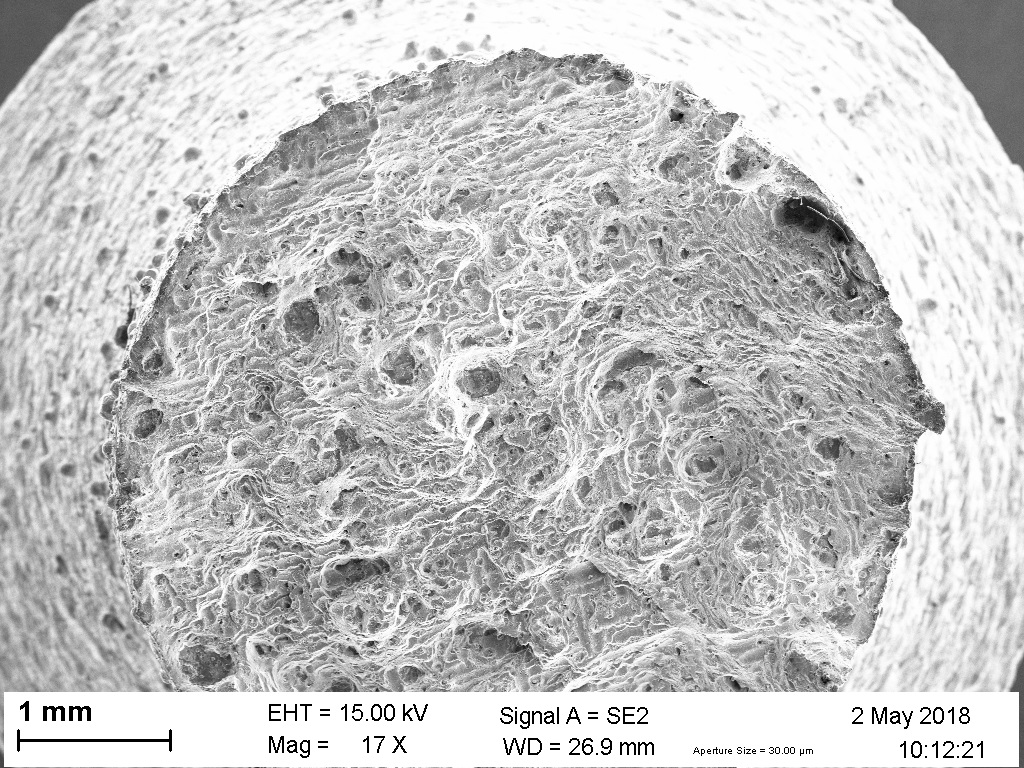
\includegraphics[scale=0.40]{Images/frac-04_01.jpg}}
	\decoRule
	\caption[Fractograph of a 300$^\circ$C-2h tensile sample]{Fractograph of a 300$^\circ$C-2h tensile sample.}
	\label{fig:frac_04_01}
\end{figure}

\begin{figure}[ht]
	\centering
	\centerline{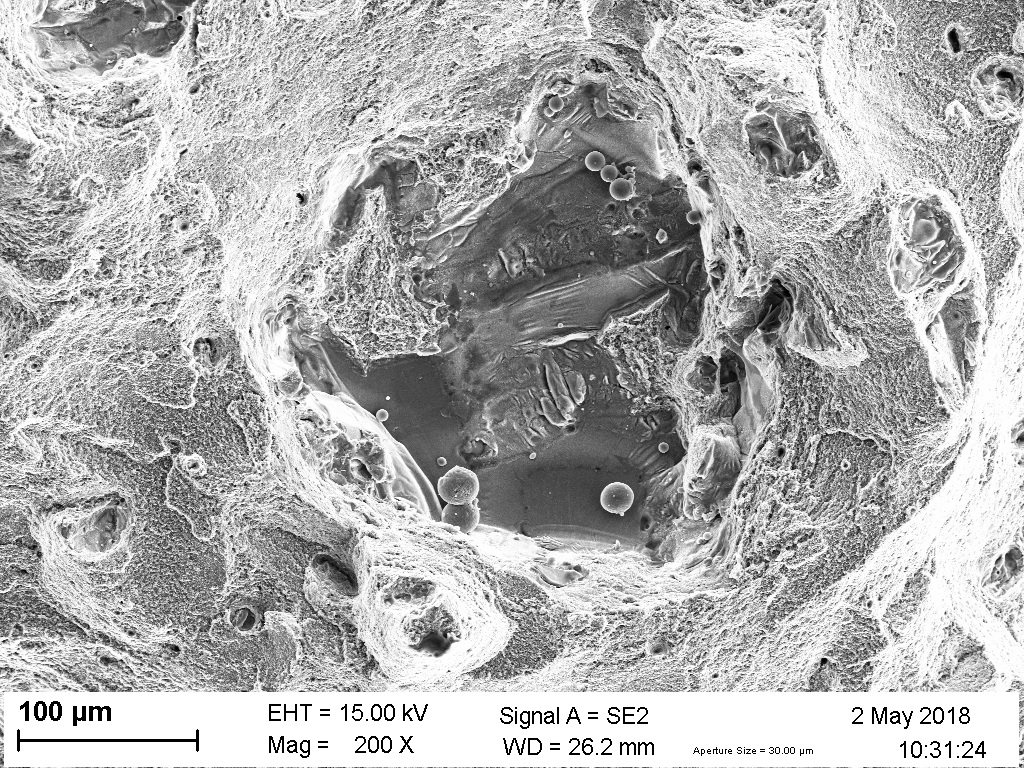
\includegraphics[scale=0.40]{Images/frac-04_11.jpg}}
	\decoRule
	\caption[View of the smooth fracture surface of 300$^\circ$C-2h sample. A couple unmelted powder particles are visible]{View of the smooth fracture surface of 300$^\circ$C-2h sample. A couple unmelted powder particles are visible.}
	\label{fig:frac_04_11}
\end{figure}

\begin{figure}[ht]
	\centering
	\centerline{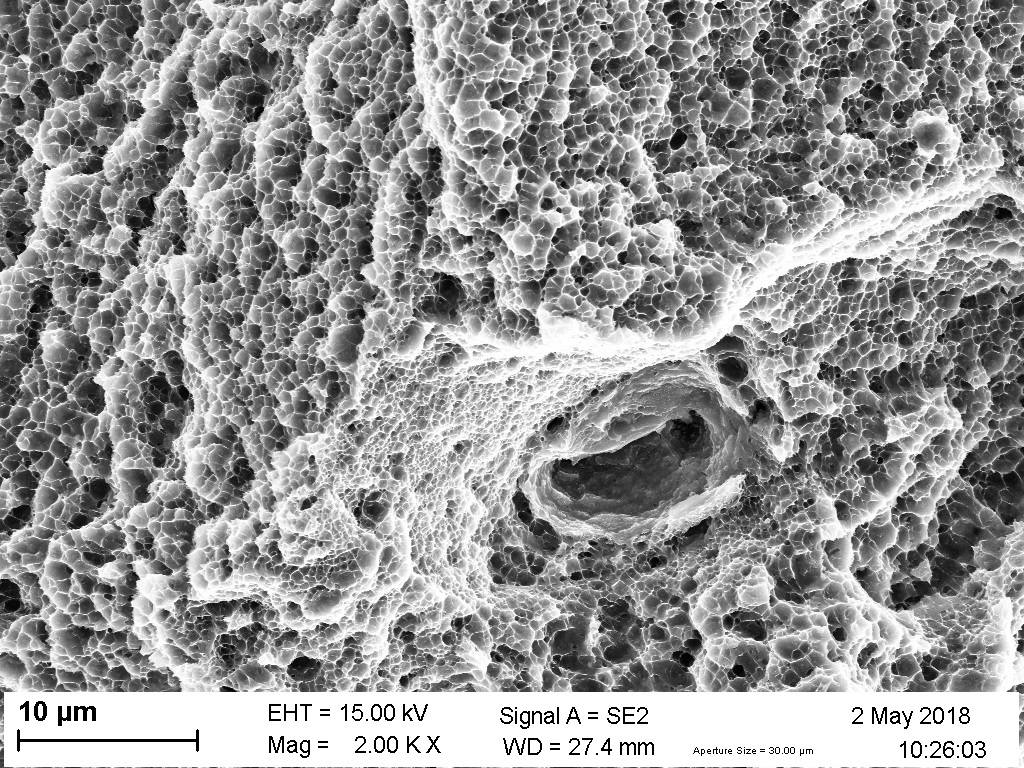
\includegraphics[scale=0.40]{Images/frac-04_08.jpg}}
	\decoRule
	\caption[Close-up shot on the ductile dimples of the 300$^\circ$C-2h sample fracture surface]{Close-up shot on the ductile dimples of the 300$^\circ$C-2h sample fracture surface.}
	\label{fig:frac_04_08}
\end{figure}

\begin{figure}[ht]
	\centering
	\centerline{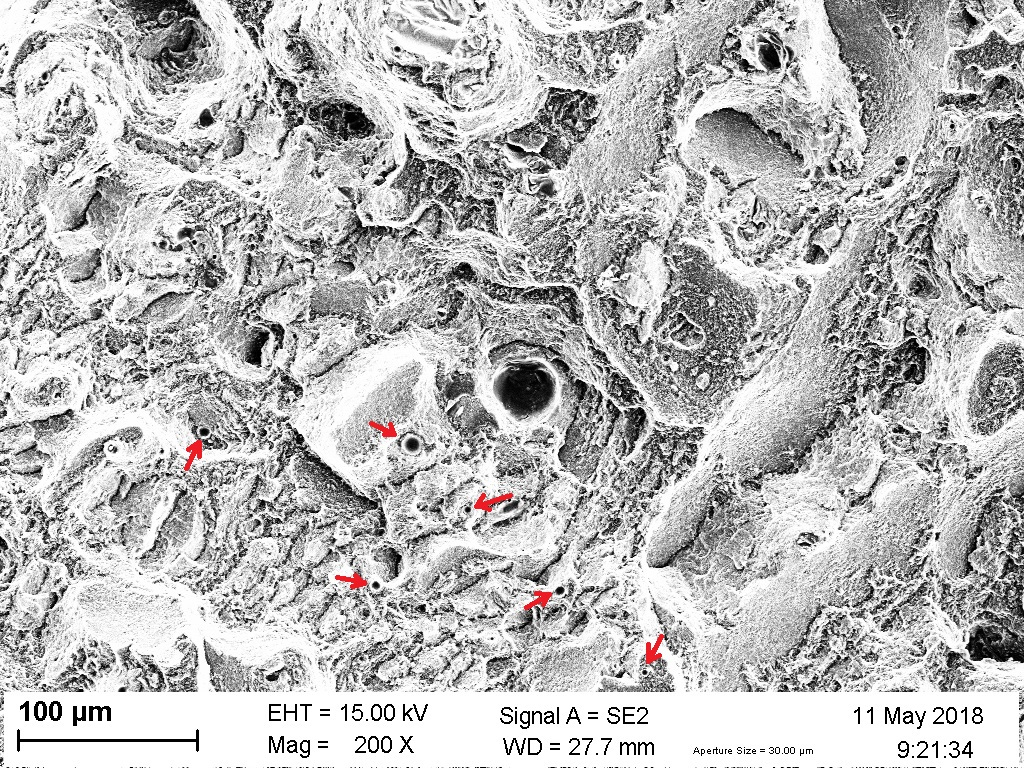
\includegraphics[scale=0.40]{Images/frac-10_26.jpg}}
	\decoRule
	\caption[View of the smooth fracture surface of 300$^\circ$C-2h sample. A couple unmelted powder particles are visible]{View of the smooth fracture surface of 300$^\circ$C-2h sample. A couple unmelted powder particles are visible.}
	\label{fig:frac_10_26}
\end{figure}

\section{Residual stresses}

X-ray diffraction of an as-built sample cut in half gave the Fig. \ref{fig:XRD} as a result. A zoom on the main aluminium peak (around 38.4$^\circ$) \cite{Rosenthal14}, including comparison with the various heat-treated samples, is available in Fig. \ref{fig:XRD_zoom}. The value of full width at half-maximum (FWHM) for all 5 samples is available in Table \ref{tab:fwhm}.

\begin{figure}[ht]
	\centering
	\centerline{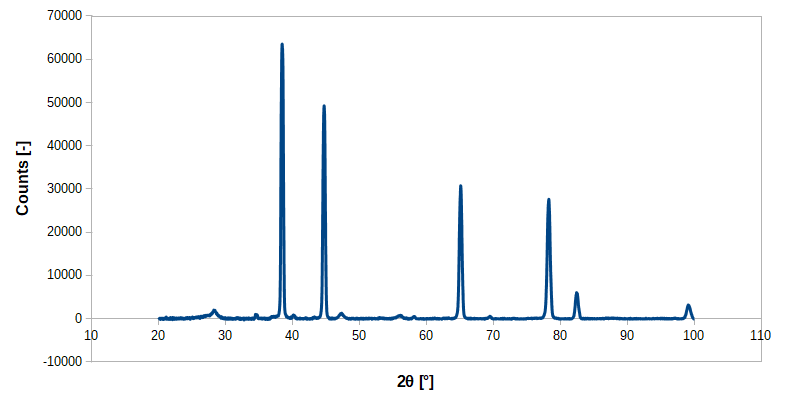
\includegraphics[scale=0.60]{Images/XRD}}
	\decoRule
	\caption[X-Ray diffractogram of a X200-180109 as-built sample]{X-Ray diffractogram of a X200-180109 as-built sample.}
	\label{fig:XRD}
\end{figure}

\begin{figure}[ht]
	\centering
	\centerline{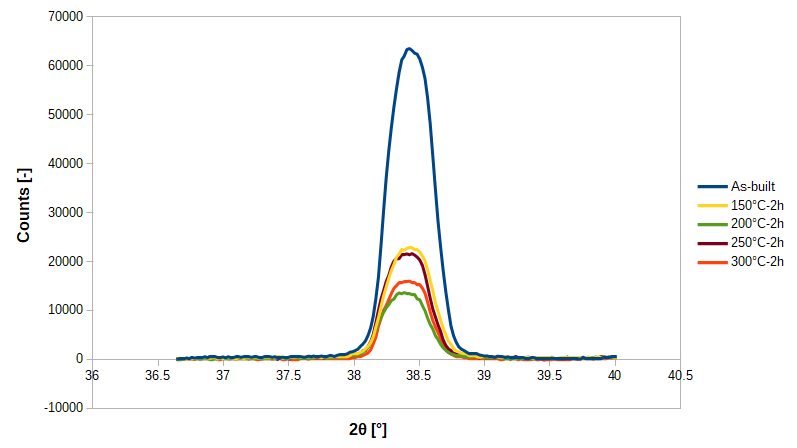
\includegraphics[scale=0.60]{Images/XRD_zoom}}
	\decoRule
	\caption[Close-up view on the highest Al peak, for the 5 different samples]{Close-up view on the highest Al peak, for the 5 different samples.}
	\label{fig:XRD_zoom}
\end{figure}

\begin{center}
	\begin{table}[ht]
		\noindent\makebox[\textwidth]{\begin{tabular}{|c |c |c| c|c|c|}
				\hline
				Sample & As-built & 150$^\circ$-2h & 200$^\circ$-2h & 250$^\circ$-2h & 300$^\circ$-2h \\
				
				\hline   
				FWHM [$^\circ$] & 0.402 & 0.410 & 0.408 & 0.402 & 0.400 \\
				
				\hline
		\end{tabular}}
	
	\caption[Full width at half-maximum for the cut as-built sample and the 4 cubix heat-treated samples]{Average tensile mechanical properties of the as-built specimens from batch X200-180417}
	\label{tab:fwhm}
\end{table}
\end{center}

Hole-drilling method gives more quantitative results. When we assume that the residual stresses are uniform along the xy planes, at least at the scale of the hole, we obtain that the as-built sample present a maximal and minimal principal stress respectively of 10 and 1 MPa. For the sample heat-treated at 300$^\circ$C for 2h, they are 43 and 23 MPa. On the other hand, when the assumption that stress varies depending on the depth, the two chosen calculation methods offer different results, available in Fig. \ref{fig:result_rs1}.

\begin{figure}[ht]
	\centering
	\centerline{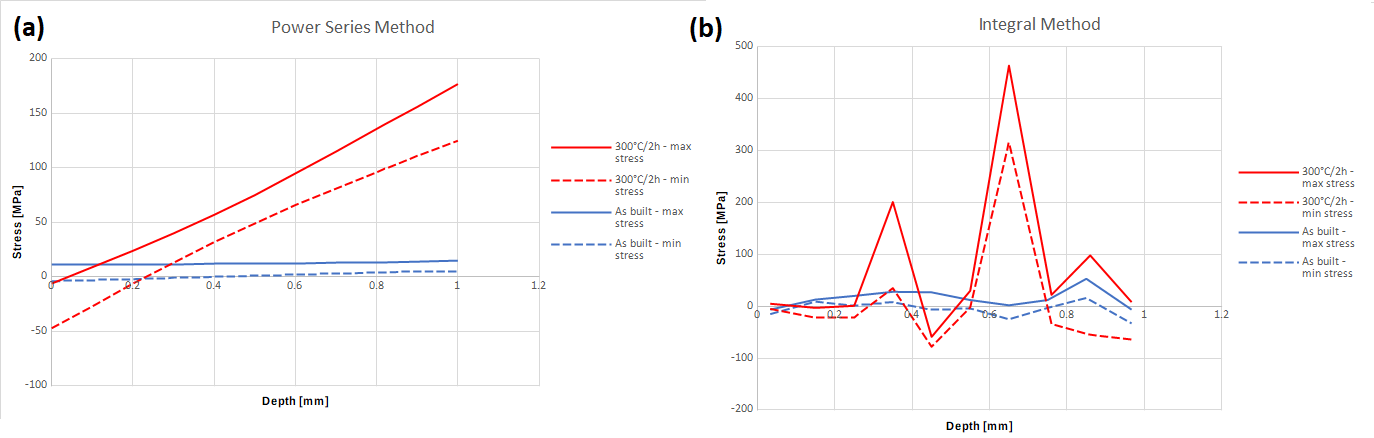
\includegraphics[scale=0.60]{Images/result_rs1}}
	\decoRule
	\caption[Magnitude of principal residual stresses along depth in both the 300$^\circ$C-2h and the as-built sample, calculated with (a) the power series method, (b) the integral method]{Magnitude of principal residual stresses along depth in both the 300$^\circ$C-2h and the as-built sample, calculated with (a) the power series method, (b) the integral method.}
	\label{fig:result_rs1}
\end{figure}